\documentclass[12pt,a4paper]{article}
\usepackage[utf8]{inputenc}
% packages
\usepackage{amsmath}
\usepackage{amsfonts}
\usepackage{amssymb}
\usepackage{graphicx}
\usepackage{listings}
\usepackage{booktabs}
\usepackage{longtable}
\usepackage[table,xcdraw]{xcolor}
\usepackage{color}
\usepackage{lscape}
\usepackage{multirow}
\usepackage{caption}
\captionsetup[table]{labelfont=bf,textfont=normalfont,singlelinecheck=on,justification=raggedright}
\definecolor{pblue}{rgb}{0.13,0.13,1}
\definecolor{pgreen}{rgb}{0,0.5,0}
\definecolor{pred}{rgb}{0.9,0,0}
\definecolor{pgrey}{rgb}{0.46,0.45,0.48}
\lstset{ %
language=Java,                % choose the language of the code
basicstyle=\footnotesize,       % the size of the fonts that are used for the code
numbers=left,                   % where to put the line-numbers
numberstyle=\footnotesize,      % the size of the fonts that are used for the line-numbers
stepnumber=1,                   % the step between two line-numbers. If it is 1 each line will be numbered
commentstyle=\color{pgreen},
keywordstyle=\color{pblue},
stringstyle=\color{pred},
numbersep=5pt,                  % how far the line-numbers are from the code
backgroundcolor=\color{white},  % choose the background color. You must add \usepackage{color}
showspaces=false,               % show spaces adding particular underscores
showstringspaces=false,         % underline spaces within strings
showtabs=false,                 % show tabs within strings adding particular underscores
frame=single,           % adds a frame around the code
tabsize=2,          % sets default tabsize to 2 spaces
captionpos=b,           % sets the caption-position to bottom
breaklines=true,        % sets automatic line breaking
breakatwhitespace=false,    % sets if automatic breaks should only happen at whitespace
escapeinside={\%*}{*)}          % if you want to add a comment within your code
}

\begin{document}

\begin{titlepage} % Suppresses displaying the page number on the title page and the subsequent page counts as page 1
	\newcommand{\HRule}{\rule{\linewidth}{0.5mm}} % Defines a new command for horizontal lines, change thickness here
	
	\center
	\textsc{\LARGE Galway Mayo Institute of Technology}\\[1.5cm] 
	\textsc{\Large H. Dip in Science \\(Software and Computing)}\\[0.5cm] % Major heading such as course name
	\textsc{\large Computational Thinking and Algorithms}\\[0.5cm] % Minor heading such as course title	
	\HRule\\[0.4cm]
	
	{\huge\bfseries Benchmarking Sorting Algorithms in Java}\\[0.4cm] % Title of your document
	
	\HRule\\[1.5cm]
	\begin{minipage}{0.4\textwidth}
		\begin{flushleft}
			\large
			\textit{Author}\\
			Kieran P. \textsc{Somers} % Your name
		\end{flushleft}
	\end{minipage}
	~
	\begin{minipage}{0.4\textwidth}
		\begin{flushright}
			\large
			\textit{Lecturer}\\
			Dr. Dominic \textsc{Carr} % Supervisor's name
		\end{flushright}
	\end{minipage}

	\vfill\vfill\vfill % Position the date 3/4 down the remaining page
	
	{\large\today} % Date, change the \today to a set date if you want to be precise
	\vfill % Push the date up 1/4 of the remaining page
	
\end{titlepage}

\section{Introduction}
``Data is the new oil'' -- in 2017 \emph{The Economist} reported that the World's most valuable resource was no longer petroleum \cite{economist, bhageshpur_council_nodate}. We are entering the age of the 4$^{th}$ Industrial Revolution \cite{schwab_fourth_2016}, an era characterised by the convergence of technologies, biologies, and societies and one which is forecast to change the way in which individuals live and work, and the way in which entire societies and economies operate and interact. Indeed one can hardly go a day without encountering a popular science or news article reporting on the latest breakthroughs facilitated by ``Big Data'', ``AI'', ``Smart Devices'', or the ``Internet of Things''. 

At both the forefront and foundations of this new era is information technology, its central role cemented by advances in materials and hardware -- from small scale wearable devices, to massively parallel Exascale computing infrastructures \cite{aurora}, to the development of the first generation of commercial quantum computers \cite{ibm}. In parallel with these physical advances, are advances in the software we use to exploit available computing power -- be it to improve our social experiences \emph{via} the latest applications and games, or the development of advanced numerical scientific libraries optimised for novel tensor-processing-units (TPUs) \cite{tpu} to be used in machine-learning and AI applications. There is no doubt that computational technology is developing at ever increasing rates as a result of the synergistic development of novel computational hardware and software.

Whilst developing novel hardware is largely an experimental endeavour, albeit one which is almost certainly accompanied by theory (i.e. the design of novel superconducting materials), the analysis and development of novel software and algorithms certainly requires a greater emphasis on theoretical insight, particularly when performance is important. The ability to analyse a problem in a computational manner, and transform that into an efficient and robust algorithm is a critical skill for a modern software developer. The theoretical under-pinnings of algorithm analysis and design are much too broad to consider in any detail here, rather, we will focus on gaining some entry-level insight by way of one of the most frequently occuring computational operations carried out -- the sorting of a list.

A ``greenhorn'' approach is as follows: ``Hey \textsc{Alexa}. What's the fastest way to sort a list?''. Whilst \textsc{Alexa} may offer some naive insight, if the same question were asked of two seasoned computational thinkers (i.e. programmers), they may well ponder for some time, and return some time later-again, having devised two different solutions to the same problem, each equally valid within its own set of constraints (input size, available hardware, software restrictions, etc.). What is likely, or at least what one hopes would have occured, is that both programmers have justified their approaches based on sound scientific principles -- their design has been accompanied by some formal or informal analysis, be it theoretical or empirical. In this report we will take such an approach, and analyse the performance of various sorting algorithms using both theoretical and empirical methods.

The aim of all sorting algorithms is to take some list or collection of objects, be they primitive or complex types, and to place them in some predefined order of relevance to the type. In some cases the ``natural order'' is obvious, for instance an algorithm which sorts the natural numbers would place the number 1 before the number 2, 2 before 3, etc. based on increasing numerical value. Similarly, the natural ordering of strings of text would place $a$ before $b$, $b$ before $c$ and so on, in an increasing lexicographical order. In cases where no obvious natural order emerges, the precise definition of whether a list of objects is sorted is dependent on some definition of equivalence as defined by a \emph{comparator} function, which will vary depending on the objects being compared, and the situation. For instance, the natural ordering for a collection of dogs is ambiguous, and one could sort them by age (a natural numerical ordering), name (a natural lexicographical order), color, breed, sex, or some combination of all of the above. What is important is that the definitions of equality are put in place prior to any sorting happening by the definition of \emph{some} comparator function.

Irrespective of the details of equivalence, for a sorting algorithm to be deemed functional it must typically satisfy two criteria. The first is that it places the elements in increasing order where equivalent elements are contiguous. For an array $A$ with at least two integer indices $i$ and $j$, if $i < j$ the corresponding array elements $A[i]$ and $A[j]$ must also satisfy the criteria that $A[i] \leq A[j]$ or else the array is unsorted. By the same logic an array $A$ is deemed unsorted if it contains an element $A[i] > A[j]$ where the index $i < j$. In terms of contiguity, if for an array $A$ there is an element $A[i]$ equal to an element $A[j]$, there can be no element $A[k]$ such that $i<k<j$ and $A[i] \neq A[k] \neq A[j]$. The second condition which must be satisfied when evaluating the behavour of a sorting algorithm is that given an unsorted array $A_u$, the sorted array $A_s$ must be some permutation of $A_u$ -- that is, the contents of both arrays must be the same, only arranged in a different order, and elements cannot be removed, or changed to satisfy sort criteria. 

Note the frequent use of the logical $>$, $<$ and $=$ operators which define whether two elements are less than, greater than, or equal to each other. Again the precise definition of less than, greater than, or equal to may vary depending on the task at hand. For primitive numeric types, such as $int$, $float$, and $long$ types the familiar mathematical definitions apply, and in the current work we aim to place a series of positive integers in order of increasing value, from smallest to largest.

All definitions of equality described above effectively rely on comparisons of values using the logical $>$, $<$ and $=$ operators, and these operators are employed by so-called comparison-based methods. Certain algorithms, entitled non-comparison-based methods, forego these operations entirely, and these types of algorithms are particularly useful when comparing non-numeric data, as in the dog sort example given previously. Both comparison- and non-comparison based algorithms will be considered herein.

Sorting algorithms are further differentiable by other desirable features -- their efficiency (both in terms of speed and memory, often termed their time- and space-complexity), their stability (whether logically equivalent elements remain in the same relative order pre- and post-sorting), and whether the sorting occurs ``\emph{in-place}'' or ``\emph{out-of-place}'' (whether auxiliary memory is required to perform the sort). 

Generally speaking, the perfect sorting algorithm would satisfy all of the criteria required of a functional sorting algorithm described previously but with low time- and space-complexity (indicating efficiency), in a stable manner (if required), and the sorting would take in-place such that memory-usage is minimized. As we will see, trade-offs must be struck between these features -- certain algorithms outperform others on some of these properties, but typically not all of them, and algorithms tend to be chosen based on their overall performance which is likely based on a combination of the above factors, and the hardware which is available.

One issue which arises with respect to benchmarking sorting algorithms is experimental design. Assuming that the algorithm, input size, and programming languages are constants, differences in hardware (chip speed, memory size and bandwidth) can easily lead to factors of two or greater differences in the time required to sort a list of items. Similarly, for a given input size and set of hardware, an algorithm written in low-level or compiled languages such as \textsc{Fortran}, \textsc{C++} or \textsc{Java} is quite likely to outperform higher-level or interpreted languages such as \textsc{perl}, \textsc{Javascript}, and \textsc{Python}. Of course, not only do hardware and software influence how a piece of software performs, but if these are both assumed to be constant one must then consider the size of the input provided to the algorithm -- an algorithm which provides pleasing performance when operating on 10 inputs, may not provide such pleasant results when tasked with millions, or even hundreds, of inputs.

With so many variables at play, the question arises as to how one can objectively measure which algorithms are better than others? In order to do so, idealised approaches which are hardware and software agnostic, are required to analyse different algorithms. The most common of these is the $\mathcal{O}$($n$) or ``Big-O'' analysis, sometimes referred to as Bachmann-Landau notation \cite{bachmann_analytische_1894, landau_handbuch_1909} after its inventors, where $\mathcal{O}$ implies the order-of-magnitude performance of an algorithm for an input size, $n$. This report will carry out such an analysis, with the aims being effectively three-fold:

\begin{enumerate}
\item to analyse a number of different sorting algorithms from a theoretical perspective in order to understand and model their limiting behaviours, and to thus classify in terms of time- and space-complexity ($\mathcal{O}$-notation), stability, and whether they are in-place
\item to implement these algorithms in a modern object-orientated software development language (Java) such that one can practically employ them to sort arbitrary-sized arrays of integers
\item to empirically benchmark the performance of each algorithm by measuring their time-efficiencies for arrays of varying size, and to analyse and discuss these empirical results in light of item 1 above
\end{enumerate}

Each algorithm will now be conceptually and procedurally described, specific examples will be provided to illustrate their features, time- and space-complexities will be analysed, along with descriptions of other desirable featuresa alluded to above. Subsequent sections will then discuss how these algorithms were implemented in a Java application such that meaningful benchmark results could be obtained. In the final section the benchmark results obtained will be presented and discussed for each algorithm, and different algorithms will be compared and contrasted in light of the above. In terms of analysis of algorithms, their complexities, and numerous derivations and approximations presented in the text, no single authoritative source could be found, and a number of sources proved useful throughout the project including the module course notes \cite{mannionBubbleSort} and recommended text books \cite{harel_algorithmics_2004, heineman_algorithms_2009}, StackOverflow \cite{stack} and indeed Wikipedia \cite{wiki}. Where algorithms have been adopted from the literature, their sources are specifically acknowledged in the text.

\section{Sorting Algorithms}

\subsection{Simple comparison-based sort: BubbleSort}
BubbleSort is amongst the simplest sorting algorithms that exist, and although too slow for most practical applications, its simplicity in terms of its conceptual approach, and its programmatic implementation, make it a useful entry point for understanding sorting algorithm performance. Whilst likely in use as early as the 1950's, the first explicit usage of the term ``BubbleSort'' can be attributed to Iverson in 1962 \cite{iverson_programming_1962}, the algorithm getting its name from the fact the largest value ``bubbles'' towards the top, or end, of the array as the array is traversed and individual elements are sorted. It is an ``in-place'' algorithm -- it requires a constant amount of auxiliary memory to perform the sort, irrespective of array size, and it is also stable in that the order of equivalent elements are preserved. As a comparison-based sorting method, it uses only logical comparison based operations ($<$, $>$) to determine whether elements are in the desired order.

The BubbleSort algorithm implemented in Java in the current project has been adapted from the course notes of Mannion \cite{mannionBubbleSort}. The adapted source code is given in Listing \ref{bubbleSortSource}, and a diagramatic representation is provided in Table \ref{bubbleSortDiagram}. 

The BubbleSort procedure relies on two loops, an outer loop and a nested inner loop, with the inner loop responsible for testing the array elements such that for indices $j$ and $j+1$, $A[j] < A[j+1]$. The outer loop iterates through the array in descending order of elements, reducing its starting value defined by the index $i$ by 1 unit per iteration. The outer loop therefore defines an upper bound for testing during the execution of the inner loop, which sequentially examines all pairs of elements at indices $j$ and $j+1$, for values of $j$ from $j = 0$ to $j < i$. Procedurally, the approach can be described as follows:

\begin{enumerate}
	\item initialize the outer loop with index $i$ equal to the last index in the array (the array length minus 1)
	\item initialize the inner loop, with index $j$ equal to the first index in the array (0)
	\item if $A[j] > A[j+1]$, swap the two values such that $A[j] < A[j+1]$
	\item increment the counter $j$ and repeat step 3 for all indices $j < i$
	\item when $j$ is equal to $i-1$ terminate the inner loop. At this point:
	\begin{itemize}
		\item the largest value between index 0 and $i$ has now been put in place at index $i$
	\end{itemize}
	\item decrement the counter $i$, and repeat steps $2-5$ until the exit condition for the outer loop is met ($i =  1$).
\end{enumerate}

Note that with respect to Step 3 above, and line 16 in Listing \ref{bubbleSortSource} below BubbleSort can be deemed ``stable'' -- that is, if two sequential elements, $A[j]$ and $A[j+1]$, have the same value they will not be swapped, and so BubbleSort preserves the original ordering of same-valued elements.

\clearpage



\begin{lstlisting}[caption={Implementation of a basic Bubblesort algorithm in Java \cite{mannionBubbleSort}. Note that there is no logic to terminate the sort procedure for an array that is already sorted.},captionpos=b, label={bubbleSortSource}]
public static void iterativeBubbleSort(int[] array) {

	// outer array starts at last index of array
	// and decrements while it is greater than 0
	for (int i = array.length - 1; i > 0; i--) {

		// inner loop starts at first index of array
		// and increases while it is less than i
		// it will terminate therefore when i = 1, and j = 0
		for (int j = 0; j < i; j++) {
		
			// if the value of array[j] > than next element in array
			// push the j value into a temp array
			// then swap element j+1 which is smaller than element j
			// with element j, which is greater
			if (array[j] > array[j + 1]) {
				int temp = array[j];
				array[j] = array[j + 1];
				array[j + 1] = temp;
			}
		}
	}
}
\end{lstlisting}

Table \ref{bubbleSortDiagram} shows the sort procedure for a simple array of $n$ = 5 elements, [5,3,6,4,1], which has a total of 7 inversions: [5,3], [5,4], [5,1], [6,4], [6,1], [3,1], and [4,1].

In terms of time complexity the outer loop indexed by $i$ runs a total of $n-1$ times. The inner loop indexed by $j$ runs $n-2$ times on the first iteration, $n-3$ times on the second iteration, etc, until it runs a total of once on the final iteration. 

The total number of iterations can be computed as the sum of the iterations of the inner loop, a sequence which corresponds to a sum of natural numbers (4+3+2+1), leading to a triangular number (10), whose value can be computed analytically from the number of elements in the array as $n(n-1)/2$, or $(n^2-n)/2$. 

Within the inner loop there are a number of constant time operations -- the greater than operation within the $if$ statment, and three three subsequent value assignments for $temp$, $array[j]$ and $array[j+1]$. Within $\mathcal{O}$ notation, these constant time operations and terms are ignored, thus leading to the well-known average-case, $\Theta$, and worst-case, $\mathcal{O}$, time-complexities of Bubble Sort of $\approx$ $n^2$. 

In the best-case scenario, Bubble Sort is known to have a time complexity, $\Omega$ = $n$ for an array that is already sorted, i.e. $A = [1,2,3,4,5]$, and therefore one which has no inversions. Note that the algorithm presented in Listing \ref{bubbleSortSource} does not account for this and will perform $(n^2-n)/2$ operations irrespective of whether the array is already sorted. 

This can be remedied \emph{via} the alterations presented in Listing \ref{bubbleSortSource2}, which includes specific logic to count the number of swap operations performed (these operations are constant time and so can be neglected in ``Big-O'' determinations). In the event that a sorted array is provided as input and no inversions are present in the array over a complete a series of iterations of the inner loop, the implementation in Listing \ref{bubbleSortSource2} will terminate after $\approx$ $n$ iterations over the inner loop, and one iteration over the outer loop, thus leading to the best-case performance of BubbleSort of $\Theta$($n$).

With respect to the space-complexity of BubbleSort, and ignoring the memory required to store the \emph{IntegerSorter} instance class and its methods -- memory is required to store $n$ array elements, 2 $int$ types in the $for$ loops ($i$ and $j$), and 1 temporary variables ($int$ $temp$) to perform the swap. The memory required to store the $n$ array elements can effectively be ignore, and only the extra, or auxiliary, memory should be considered. In such a case the extra memory required is effectively constant, and is independent of $n$, leading to a space-complexity of $\mathcal{O}$(1) for the algorithm shown in Listing \ref{bubbleSortSource}. For the algorithm show in Listing \ref{bubbleSortSource2} more memory is required to store a single extra integer, $numberInversion$, although this is a minor burden in terms of memory requirements and $\mathcal{O}$(1) space complexity still applies. Overall the space-complexity of BubbleSort, along with its simplicity, are amongst its only positive features -- as we will see its performance is less than desirable for arrays of any meaningful size given its $n^2$ average and worst case time-complexity.

\clearpage

\begin{lstlisting}[caption={Modification of the iterative bubble sort algorithm \cite{mannionBubbleSort} to account for a best case scenario where no inversions are present.},captionpos=b, label={bubbleSortSource2}]
public static void iterativeBubbleSort(int[] array) {

	// add a variable to count the number
	// of inversions carried out
	int numberInversion = 0;

	// outer array starts at last index of array
	// and decrements while it is greater than 0
	
	for (int i = array.length - 1; i > 0; i--) {

		// inner loop starts at first index of array
		// and increases while it is less than i
		// it will terminate therefore when i = 1, and j = 0
		// if the value of array[j] > than next element in array
		// push the j value into a temp array, then swap element j+1
		// which is smaller than element j, with element j, which is greater
		for (int j = 0; j < i; j++) {
			if (array[j] > array[j + 1]) {
				numberInversion++;
				int temp = array[j];
				array[j] = array[j + 1];
				array[j + 1] = temp;
			}
		}

		// if the number of inversions
		// is zero the array is already sorted
		// and so the outer loop should break
		// this will give best case O(n)
		// running time for a pre-sorted array
		if (numberInversion == 0) {
			break;
		}
	}
}
\end{lstlisting}

\clearpage


\begin{landscape}
\begin{table}[]
\begin{center}

\begin{tabular}{|c|c|c|c|c|c|c|
>{\columncolor[HTML]{34FF34}}c |c|}
\hline
\cellcolor[HTML]{FFFFFF}{\color[HTML]{000000} \textbf{iteration}} & \cellcolor[HTML]{FFFFFF}{\color[HTML]{000000} \textit{\textbf{i}}} & \cellcolor[HTML]{FFFFFF}{\color[HTML]{000000} \textit{\textbf{j}}} & \cellcolor[HTML]{FFFFFF}{\color[HTML]{000000} \textbf{arr{[}0{]}}} & \cellcolor[HTML]{FFFFFF}{\color[HTML]{000000} \textbf{arr{[}1{]}}} & \cellcolor[HTML]{FFFFFF}{\color[HTML]{000000} \textbf{arr{[}2{]}}} & \cellcolor[HTML]{FFFFFF}{\color[HTML]{000000} \textbf{arr{[}3{]}}} & \cellcolor[HTML]{FFFFFF}{\color[HTML]{000000} \textbf{arr{[}4{]}}} & {\color[HTML]{000000} \textit{\textbf{action/comment}}}                  \\ \hline
\cellcolor[HTML]{FFFFFF}{\color[HTML]{000000} \textit{1}}         & \cellcolor[HTML]{FFFFFF}{\color[HTML]{000000} \textit{4}}          & \cellcolor[HTML]{FFFFFF}{\color[HTML]{000000} \textit{0}}          & \cellcolor[HTML]{C0C0C0}{\color[HTML]{000000} 5}                   & \cellcolor[HTML]{C0C0C0}{\color[HTML]{000000} 3}                   & \cellcolor[HTML]{FFFFFF}{\color[HTML]{000000} 6}                   & \cellcolor[HTML]{FFFFFF}{\color[HTML]{000000} 4}                   & \cellcolor[HTML]{656565}{\color[HTML]{000000} 1}                   & {\color[HTML]{000000} \textit{compare, swap}}                            \\ \hline
\cellcolor[HTML]{FFFFFF}{\color[HTML]{000000} \textit{2}}         & \cellcolor[HTML]{FFFFFF}{\color[HTML]{000000} \textit{4}}          & \cellcolor[HTML]{FFFFFF}{\color[HTML]{000000} \textit{1}}          & \cellcolor[HTML]{FFFFFF}{\color[HTML]{000000} 3}                   & \cellcolor[HTML]{C0C0C0}{\color[HTML]{000000} 5}                   & \cellcolor[HTML]{C0C0C0}{\color[HTML]{000000} 6}                   & \cellcolor[HTML]{FFFFFF}{\color[HTML]{000000} 4}                   & \cellcolor[HTML]{656565}{\color[HTML]{000000} 1}                   & {\color[HTML]{000000} \textit{compare, don't swap}}                      \\ \hline
\cellcolor[HTML]{FFFFFF}{\color[HTML]{000000} \textit{3}}         & \cellcolor[HTML]{FFFFFF}{\color[HTML]{000000} \textit{4}}          & \cellcolor[HTML]{FFFFFF}{\color[HTML]{000000} \textit{2}}          & \cellcolor[HTML]{FFFFFF}{\color[HTML]{000000} 3}                   & \cellcolor[HTML]{FFFFFF}{\color[HTML]{000000} 5}                   & \cellcolor[HTML]{C0C0C0}{\color[HTML]{000000} 6}                   & \cellcolor[HTML]{C0C0C0}{\color[HTML]{000000} 4}                   & \cellcolor[HTML]{656565}{\color[HTML]{000000} 1}                   & {\color[HTML]{000000} \textit{compare, swap}}                            \\ \hline
\cellcolor[HTML]{FFFFFF}{\color[HTML]{000000} \textit{4}}         & \cellcolor[HTML]{FFFFFF}{\color[HTML]{000000} \textit{4}}          & \cellcolor[HTML]{FFFFFF}{\color[HTML]{000000} \textit{3}}          & \cellcolor[HTML]{FFFFFF}{\color[HTML]{000000} 3}                   & \cellcolor[HTML]{FFFFFF}{\color[HTML]{000000} 5}                   & \cellcolor[HTML]{FFFFFF}{\color[HTML]{000000} 4}                   & \cellcolor[HTML]{C0C0C0}{\color[HTML]{000000} 6}                   & \cellcolor[HTML]{C0C0C0}{\color[HTML]{000000} 1}                   & {\color[HTML]{000000} \textit{compare, swap}}                            \\ \hline
\cellcolor[HTML]{FFFFFF}{\color[HTML]{000000} \textit{N/A}}       & \cellcolor[HTML]{FFFFFF}{\color[HTML]{000000} \textit{}}           & \cellcolor[HTML]{FFFFFF}{\color[HTML]{000000} \textit{}}           & \cellcolor[HTML]{FFFFFF}{\color[HTML]{000000} 3}                   & \cellcolor[HTML]{FFFFFF}{\color[HTML]{000000} 5}                   & \cellcolor[HTML]{FFFFFF}{\color[HTML]{000000} 4}                   & \cellcolor[HTML]{FFFFFF}{\color[HTML]{000000} 1}                   & {\color[HTML]{000000} 6}                                           & {\color[HTML]{000000} \textit{one element sorted; i = i - 1; j = 0;}}    \\ \hline
\cellcolor[HTML]{FFFFFF}{\color[HTML]{000000} \textit{5}}         & \cellcolor[HTML]{FFFFFF}{\color[HTML]{000000} \textit{3}}          & \cellcolor[HTML]{FFFFFF}{\color[HTML]{000000} \textit{0}}          & \cellcolor[HTML]{C0C0C0}{\color[HTML]{000000} 3}                   & \cellcolor[HTML]{C0C0C0}{\color[HTML]{000000} 5}                   & \cellcolor[HTML]{FFFFFF}{\color[HTML]{000000} 4}                   & \cellcolor[HTML]{656565}{\color[HTML]{000000} 1}                   & {\color[HTML]{000000} 6}                                           & {\color[HTML]{000000} \textit{compare, don't swap}}                      \\ \hline
{\color[HTML]{000000} \textit{6}}                                 & {\color[HTML]{000000} \textit{3}}                                  & {\color[HTML]{000000} \textit{1}}                                  & {\color[HTML]{000000} 3}                                           & \cellcolor[HTML]{C0C0C0}{\color[HTML]{000000} 5}                   & \cellcolor[HTML]{C0C0C0}{\color[HTML]{000000} 4}                   & \cellcolor[HTML]{656565}{\color[HTML]{000000} 1}                   & {\color[HTML]{000000} 6}                                           & {\color[HTML]{000000} \textit{compare, swap}}                            \\ \hline
{\color[HTML]{000000} \textit{7}}                                 & {\color[HTML]{000000} \textit{3}}                                  & {\color[HTML]{000000} \textit{2}}                                  & {\color[HTML]{000000} 3}                                           & {\color[HTML]{000000} 4}                                           & \cellcolor[HTML]{C0C0C0}{\color[HTML]{000000} 5}                   & \cellcolor[HTML]{C0C0C0}{\color[HTML]{000000} 1}                   & {\color[HTML]{000000} 6}                                           & {\color[HTML]{000000} \textit{compare, swap}}                            \\ \hline
{\color[HTML]{000000} \textit{N/A}}                               & {\color[HTML]{000000} \textit{}}                                   & {\color[HTML]{000000} }                                            & {\color[HTML]{000000} 3}                                           & {\color[HTML]{000000} 4}                                           & {\color[HTML]{000000} 1}                                           & \cellcolor[HTML]{34FF34}{\color[HTML]{000000} 5}                   & {\color[HTML]{000000} 6}                                           & {\color[HTML]{000000} \textit{two elements sorted; i = i - 1; j = 0;}}   \\ \hline
{\color[HTML]{000000} \textit{8}}                                 & {\color[HTML]{000000} \textit{2}}                                  & {\color[HTML]{000000} \textit{0}}                                  & \cellcolor[HTML]{C0C0C0}{\color[HTML]{000000} 3}                   & \cellcolor[HTML]{C0C0C0}{\color[HTML]{000000} 4}                   & {\color[HTML]{000000} 1}                                           & \cellcolor[HTML]{34FF34}{\color[HTML]{000000} 5}                   & {\color[HTML]{000000} 6}                                           & {\color[HTML]{000000} \textit{compare, don't swap}}                      \\ \hline
{\color[HTML]{000000} \textit{9}}                                 & {\color[HTML]{000000} \textit{2}}                                  & {\color[HTML]{000000} \textit{1}}                                  & {\color[HTML]{000000} 3}                                           & \cellcolor[HTML]{C0C0C0}{\color[HTML]{000000} 4}                   & \cellcolor[HTML]{C0C0C0}{\color[HTML]{000000} 1}                   & \cellcolor[HTML]{34FF34}{\color[HTML]{000000} 5}                   & {\color[HTML]{000000} 6}                                           & {\color[HTML]{000000} \textit{compare, swap}}                            \\ \hline
{\color[HTML]{000000} \textit{N/A}}                               & {\color[HTML]{000000} }                                            & {\color[HTML]{000000} }                                            & {\color[HTML]{000000} 3}                                           & {\color[HTML]{000000} 1}                                           & \cellcolor[HTML]{34FF34}{\color[HTML]{000000} 4}                   & \cellcolor[HTML]{34FF34}{\color[HTML]{000000} 5}                   & {\color[HTML]{000000} 6}                                           & {\color[HTML]{000000} \textit{three elements sorted; i = i - 1; j = 0;}} \\ \hline
{\color[HTML]{000000} \textit{10}}                                & {\color[HTML]{000000} \textit{1}}                                  & {\color[HTML]{000000} \textit{0}}                                  & \cellcolor[HTML]{C0C0C0}{\color[HTML]{000000} 3}                   & \cellcolor[HTML]{C0C0C0}{\color[HTML]{000000} 1}                   & \cellcolor[HTML]{34FF34}{\color[HTML]{000000} 4}                   & \cellcolor[HTML]{34FF34}{\color[HTML]{000000} 5}                   & {\color[HTML]{000000} 6}                                           & {\color[HTML]{000000} \textit{compare, swap}}                            \\ \hline
{\color[HTML]{000000} \textit{exit}}                              & {\color[HTML]{000000} }                                            & {\color[HTML]{000000} }                                            & \cellcolor[HTML]{34FF34}{\color[HTML]{000000} 1}                   & \cellcolor[HTML]{34FF34}{\color[HTML]{000000} 3}                   & \cellcolor[HTML]{34FF34}{\color[HTML]{000000} 4}                   & \cellcolor[HTML]{34FF34}{\color[HTML]{000000} 5}                   & {\color[HTML]{000000} 6}                                           & {\color[HTML]{000000} \textit{all elements sorted; exit}}                \\ \hline
\end{tabular}
\caption{Table illustrating the BubbleSort procedure for an array of 5 elements: [5, 3, 6, 4, 1]. Iterations, and values for the indices $i$ and $j$ are enumerated in the first three columns. Values for each array element at each iteration are in columns $4-8$. Cells in light grey correspond to two elements current being compared. Cells in dark grey correspond to the current index of $i$ (the last element which will be compared), unless the element at index $i$ is being compared, in which case it is highlighed in light grey. Elements which have been sorted are highlighted in green cells. Comments are outlined in the right most column. This diagram was generated by the author \emph{via} an online \LaTeX table generator \cite{latexTableGenerator}.}
\label{bubbleSortDiagram}
\end{center}
\end{table}
\end{landscape}

\clearpage

\subsection{Efficient comparison-based sort: QuickSort}
QuickSort was developed by Hoare in 1959 and published in 1961 \cite{hoare_algorithm_1961}. Like BubbleSort it is a comparison-based sort which relies only on logical comparison operators ($<$, $\leq$, $>$, $\geq$, $=$) to determine whether elements are sorted, and this sorting effectively be carried out in-place as the auxiliary memory requirements are low. However it is not guaranteed to be stable and the order of equivalent elements may not be preserved pre- and post-sorting. It is a recursive divide-and-conquer algorithm which works by splitting an array into two sub-arrays based on the value chosen for a single element which defines the boundary for the partition known as the pivot. The two sub-arrays are then recursively sorted \emph{via} the same procedure. The QuickSort algorithm implemented in this work is derived from multiple self-consistent sources  \cite{quickSort1, quickSort2, quickSort3}, and will now be described in detail.

The QuickSort algorithm can be loosely split into three steps:
\begin{enumerate}
\item selection of the pivot element
\item partitioning of values about the pivot
\item recursive sorting of the two partitions \emph{via} steps 1 and 2.
\end{enumerate}

The pivot element is an element about which other elements will be sorted -- all elements whose values are less than the pivot should be placed into the ``left'' sub-array, and all element whose values are greater than the pivot should into a seperate ``right'' sub-array. The pivot itself may exist in either. In terms of choosing an appropriate pivot, selection of the last, first, median or random elements are popular strategies. Whilst superficially the selection of the pivot appears trivial, many strategies exist to select a pivot element which leads to greatest efficiency -- for sorted, or nearly sorted arrays, selection of the last element can lead to lower efficiencies. As the arrays being sorted in the current work are all composed of randomly generated integers, the pivot element is always chosen to be the median element, whose value should also be effectively random.

The crucial step in QuickSort is the subsequent partitioning of elements. This is shown algorithmically in lines 16--45 of Listing \ref{quickSortSource} below, and schematically in Table \ref{quickSortDiagram}. The basic strategy is as follows. Given a pivot value, $P$, find an element $A[i]$ such that $A[i] \geq P$, and find an element $A[j]$ such that $A[j] \leq P$. Once the search criteria are satisfied the elements $A[i]$ are swapped if and only if $i < j$, and the search criteria is terminated if during the search $i$ becomes greater than $j$. Note that there are no restrictions on the pivot element, $A[p]$, satisfying the above criteria and being used in swaps. Algorithmically the partitioning procedure can be summarised as follows:

\begin{enumerate}
\item provide an array to be sorted, a lower sort index ($lower\_index$) and an upper sort index ($upper\_index$) with the latter two defining the limits of the search operations (the first and last elements of the array on the first call)
\item if the $lower\_index \geq upper\_index$ terminate the recursion as a base recursion condition has been met
\item define two index-counting integers $i$ and $j$ to be equal to the $lower\_index$ and $upper\_index$ respectively 
\item while the index $i$ is less than or equal to the index $j$:
\begin{enumerate}
\item search for an element $A[i] \geq P$
\item subsequently search for an element $A[j] \leq P$
\item if $i \leq j$, swap the values for $A[i]$ and $A[j]$ and increment $i$ and $j$
\end{enumerate}
\item go to step 1 with the $upper\_index =$ the current value for $j$ 
\item go to step 1 with the $lower\_index =$ the current value for $i$ 
\end{enumerate}

Note that in Listing \ref{quickSortSource} and Table \ref{quickSortDiagram} the partioning procedure leads to two distinct sub-arrays defined by the bounds $A_1[lower\_index ... j]$ and \\ $A_2[i...high\_index]$. However, new arrays are not created post-partioning or during recursive sort calls, rather, one is merely changing the lower and upper bounds of the indices used in the search- and sort-space. The algorithm can therefore be deemed in-place given that all swap operations take place on the original unsorted array and only a small amount ($\approx \log n$) of fixed memory is required to perform the sort.

In order for recursive calls to terminate such that infinite recursion is not encountered, the base condition (Listing \ref{quickSortSource} lines 5--7.) requests termination when the search-space, defined by the difference between the $lower\_index$ and $higher\_index$, is one element or less.

\clearpage


\begin{lstlisting}[caption={QuickSort algorithm \cite{quickSort1, quickSort2, quickSort3} implemented in the current project.},captionpos=b, label={quickSortSource}]
public static void quickSort(int[] array, int lower_index, int upper_index) {

	// base case: lower index >= higher index 
	// i.e. search range < 2
	if (lower_index >= upper_index) {
		return;
	}

	// get the start and end indices and set the pivot value
	// based on the median element in the array
	int i = lower_index;
	int j = upper_index;
	int pivot = array[(lower_index + upper_index) / 2];

	// iterate while the index i <= index j
	while (i <= j) {
		
		// find an element in left side 
		// whose value is greater than or equal to the pivot
		// if no larger values will stop when
		// pivot reached
		while (array[i] < pivot) {
			i++;
		}
		
		// find an element in right hand side 
		// whose value is less than or equal to the pivot
		// if no smaller values will stop when
		// pivot reached
		while (array[j] > pivot) {
			j--;
		}

		// if the index i
		// is less than or equal to
		// index j swap the two elements
		// and increment i and decrement j
		if (i <= j) {
			int temp = array[i];
			array[i] = array[j];
			array[j] = temp;
			i++;
			j--;
		}
	}

	// recursively call quick sort on 
	// array[lower_index...j]
	// and array[i...upper_index]
	IntegerSorter.quickSort(array, lower_index, j);
	IntegerSorter.quickSort(array, i, upper_index);

}
\end{lstlisting}




\clearpage
\begin{landscape}
\begin{table}[]
\begin{center}
\begin{tabular}{|c|c|c|c|c|c|c|c|c|c|}
\hline
{\color[HTML]{000000} \textit{\textbf{comment}}}                                                                                               & {\color[HTML]{000000} \textit{\textbf{arr{[}0{]}}}} & {\color[HTML]{000000} \textit{\textbf{arr{[}1{]}}}} & {\color[HTML]{000000} \textit{\textbf{arr{[}2{]}}}}       & {\color[HTML]{000000} \textit{\textbf{arr{[}3{]}}}} & {\color[HTML]{000000} \textit{\textbf{arr{[}4{]}}}}       & {\color[HTML]{000000} \textit{\textbf{arr{[}5{]}}}} & {\color[HTML]{000000} \textit{\textbf{arr{[}6{]}}}}                & {\color[HTML]{000000} \textit{\textbf{arr{[}7{]}}}} & {\color[HTML]{000000} \textit{\textbf{arr{[}8{]}}}} \\ \hline
{\color[HTML]{000000} \textit{\textbf{elements}}}                                                                                              & \cellcolor[HTML]{C0C0C0}{\color[HTML]{000000} 2}    & {\color[HTML]{000000} 1}                            & {\color[HTML]{000000} 9}                                  & {\color[HTML]{000000} 5}                            & \cellcolor[HTML]{656565}{\color[HTML]{000000} \textbf{7}} & {\color[HTML]{000000} 8}                            & {\color[HTML]{000000} 4}                                           & {\color[HTML]{000000} 6}                            & \cellcolor[HTML]{C0C0C0}{\color[HTML]{000000} 10}   \\ \hline
{\color[HTML]{000000} \textit{\textbf{index labels}}}                                                                                          & {\color[HTML]{000000} \textit{\textbf{i}}}          & {\color[HTML]{000000} }                             & {\color[HTML]{000000} }                                   & {\color[HTML]{000000} }                             & {\color[HTML]{000000} \textit{\textbf{p}}}                & {\color[HTML]{000000} }                             & {\color[HTML]{000000} }                                            & {\color[HTML]{000000} }                             & {\color[HTML]{000000} \textit{\textbf{j}}}          \\ \hline
{\color[HTML]{000000} \textit{\textbf{find arr{[}i{]} \textgreater{}= pivot}}}                                                                 & {\color[HTML]{000000} 2}                            & {\color[HTML]{000000} 1}                            & \cellcolor[HTML]{C0C0C0}{\color[HTML]{000000} 9}          & {\color[HTML]{000000} 5}                            & \cellcolor[HTML]{656565}{\color[HTML]{000000} \textbf{7}} & {\color[HTML]{000000} 8}                            & \cellcolor[HTML]{FFFFFF}{\color[HTML]{000000} 4}                   & \cellcolor[HTML]{FFFFFF}{\color[HTML]{000000} 6}    & \cellcolor[HTML]{C0C0C0}{\color[HTML]{000000} 10}   \\ \hline
{\color[HTML]{000000} \textit{\textbf{}}}                                                                                                      & {\color[HTML]{000000} }                             & {\color[HTML]{000000} }                             & {\color[HTML]{000000} \textit{\textbf{i}}}                & {\color[HTML]{000000} }                             & {\color[HTML]{000000} }                                   & {\color[HTML]{000000} }                             & {\color[HTML]{000000} }                                            & {\color[HTML]{000000} }                             & {\color[HTML]{000000} \textit{\textbf{j}}}          \\ \hline
{\color[HTML]{000000} \textit{\textbf{find arr{[}j{]} \textless{}= pivot}}}                                                                    & {\color[HTML]{000000} 2}                            & {\color[HTML]{000000} 1}                            & \cellcolor[HTML]{C0C0C0}{\color[HTML]{000000} 9}          & {\color[HTML]{000000} 5}                            & \cellcolor[HTML]{656565}{\color[HTML]{000000} \textbf{7}} & {\color[HTML]{000000} 8}                            & \cellcolor[HTML]{FFFFFF}{\color[HTML]{000000} 4}                   & \cellcolor[HTML]{C0C0C0}{\color[HTML]{000000} 6}    & {\color[HTML]{000000} 10}                           \\ \hline
{\color[HTML]{000000} \textit{\textbf{}}}                                                                                                      & {\color[HTML]{000000} }                             & {\color[HTML]{000000} }                             & {\color[HTML]{000000} \textit{\textbf{i}}}                & {\color[HTML]{000000} }                             & {\color[HTML]{000000} }                                   & {\color[HTML]{000000} }                             & {\color[HTML]{000000} \textit{\textbf{}}}                          & {\color[HTML]{000000} \textit{\textbf{j}}}          & {\color[HTML]{000000} }                             \\ \hline
{\color[HTML]{000000} \textit{\textbf{\begin{tabular}[c]{@{}c@{}}i \textless{}= j therefore swap \\ and increment i and j\end{tabular}}}}      & {\color[HTML]{000000} 2}                            & {\color[HTML]{000000} 1}                            & \cellcolor[HTML]{34FF34}{\color[HTML]{000000} 6}          & {\color[HTML]{000000} 5}                            & \cellcolor[HTML]{656565}{\color[HTML]{000000} \textbf{7}} & {\color[HTML]{000000} 8}                            & {\color[HTML]{000000} 4}                                           & \cellcolor[HTML]{34FF34}{\color[HTML]{000000} 9}    & {\color[HTML]{000000} 10}                           \\ \hline
{\color[HTML]{000000} \textit{\textbf{}}}                                                                                                      & {\color[HTML]{000000} }                             & {\color[HTML]{000000} }                             & {\color[HTML]{000000} }                                   & {\color[HTML]{000000} \textit{\textbf{i}}}          & {\color[HTML]{000000} }                                   & {\color[HTML]{000000} }                             & {\color[HTML]{000000} \textit{\textbf{j}}}                         & {\color[HTML]{000000} }                             & {\color[HTML]{000000} }                             \\ \hline
{\color[HTML]{000000} \textit{\textbf{find arr{[}i{]} \textgreater{}= pivot}}}                                                                 & {\color[HTML]{000000} 2}                            & {\color[HTML]{000000} 1}                            & \cellcolor[HTML]{34FF34}{\color[HTML]{000000} 6}          & {\color[HTML]{000000} 5}                            & \cellcolor[HTML]{C0C0C0}{\color[HTML]{000000} \textbf{7}} & {\color[HTML]{000000} 8}                            & {\color[HTML]{000000} 4}                                           & \cellcolor[HTML]{34FF34}{\color[HTML]{000000} 9}    & {\color[HTML]{000000} 10}                           \\ \hline
{\color[HTML]{000000} }                                                                                                                        & {\color[HTML]{000000} }                             & {\color[HTML]{000000} }                             & {\color[HTML]{000000} }                                   & {\color[HTML]{000000} }                             & {\color[HTML]{000000} \textit{\textbf{i}}}                & {\color[HTML]{000000} }                             & {\color[HTML]{000000} \textit{\textbf{j}}}                         & {\color[HTML]{000000} }                             & {\color[HTML]{000000} }                             \\ \hline
{\color[HTML]{000000} \textit{\textbf{find arr{[}j{]} \textless{}= pivot}}}                                                                    & {\color[HTML]{000000} 2}                            & {\color[HTML]{000000} 1}                            & \cellcolor[HTML]{34FF34}{\color[HTML]{000000} 6}          & {\color[HTML]{000000} 5}                            & \cellcolor[HTML]{C0C0C0}{\color[HTML]{000000} \textbf{7}} & {\color[HTML]{000000} 8}                            & \cellcolor[HTML]{C0C0C0}{\color[HTML]{000000} 4}                   & \cellcolor[HTML]{34FF34}{\color[HTML]{000000} 9}    & {\color[HTML]{000000} 10}                           \\ \hline
{\color[HTML]{000000} }                                                                                                                        & {\color[HTML]{000000} }                             & {\color[HTML]{000000} }                             & {\color[HTML]{000000} }                                   & {\color[HTML]{000000} }                             & {\color[HTML]{000000} \textit{\textbf{i}}}                & {\color[HTML]{000000} }                             & {\color[HTML]{000000} \textit{\textbf{j}}}                         & {\color[HTML]{000000} }                             & {\color[HTML]{000000} }                             \\ \hline
{\color[HTML]{000000} \textit{\textbf{\begin{tabular}[c]{@{}c@{}}i \textless{}= j therefore swap \\ and increment i and j\end{tabular}}}}      & {\color[HTML]{000000} 2}                            & {\color[HTML]{000000} 1}                            & \cellcolor[HTML]{34FF34}{\color[HTML]{000000} 6}          & {\color[HTML]{000000} 5}                            & \cellcolor[HTML]{34FF34}{\color[HTML]{000000} 4}          & \cellcolor[HTML]{C0C0C0}{\color[HTML]{000000} 8}    & \cellcolor[HTML]{34FF34}{\color[HTML]{000000} \textbf{7}}          & \cellcolor[HTML]{34FF34}{\color[HTML]{000000} 9}    & {\color[HTML]{000000} 10}                           \\ \hline
{\color[HTML]{000000} \textit{\textbf{}}}                                                                                                      & {\color[HTML]{000000} }                             & {\color[HTML]{000000} }                             & {\color[HTML]{000000} }                                   & {\color[HTML]{000000} }                             & {\color[HTML]{000000} }                                   & {\color[HTML]{000000} \textit{\textbf{i,j}}}        & {\color[HTML]{000000} }                                            & {\color[HTML]{000000} }                             & {\color[HTML]{000000} }                             \\ \hline
{\color[HTML]{000000} \textit{\textbf{find arr{[}i{]} \textgreater{}= pivot}}}                                                                 & {\color[HTML]{000000} 2}                            & {\color[HTML]{000000} 1}                            & \cellcolor[HTML]{34FF34}{\color[HTML]{000000} 6}          & {\color[HTML]{000000} 5}                            & \cellcolor[HTML]{34FF34}{\color[HTML]{000000} 4}          & \cellcolor[HTML]{C0C0C0}{\color[HTML]{000000} 8}    & \cellcolor[HTML]{656565}{\color[HTML]{000000} \textbf{7}}          & \cellcolor[HTML]{34FF34}{\color[HTML]{000000} 9}    & {\color[HTML]{000000} 10}                           \\ \hline
{\color[HTML]{000000} }                                                                                                                        & {\color[HTML]{000000} }                             & {\color[HTML]{000000} }                             & {\color[HTML]{000000} }                                   & {\color[HTML]{000000} }                             & {\color[HTML]{000000} }                                   & {\color[HTML]{000000} \textit{\textbf{i,j}}}        & {\color[HTML]{000000} \textit{\textbf{}}}                          & {\color[HTML]{000000} }                             & {\color[HTML]{000000} }                             \\ \hline
{\color[HTML]{000000} \textit{\textbf{find arr{[}j{]} \textless{}= pivot}}}                                                                    & {\color[HTML]{000000} 2}                            & {\color[HTML]{000000} 1}                            & \cellcolor[HTML]{34FF34}{\color[HTML]{000000} 6}          & {\color[HTML]{000000} 5}                            & \cellcolor[HTML]{C0C0C0}{\color[HTML]{000000} 4}          & \cellcolor[HTML]{C0C0C0}{\color[HTML]{000000} 8}    & \cellcolor[HTML]{656565}{\color[HTML]{000000} \textit{\textbf{7}}} & \cellcolor[HTML]{34FF34}{\color[HTML]{000000} 9}    & {\color[HTML]{000000} 10}                           \\ \hline
{\color[HTML]{000000} }                                                                                                                        & {\color[HTML]{000000} }                             & {\color[HTML]{000000} }                             & {\color[HTML]{000000} }                                   & {\color[HTML]{000000} }                             & {\color[HTML]{FE0000} \textit{\textbf{j}}}                & {\color[HTML]{FE0000} \textit{\textbf{i}}}          & {\color[HTML]{000000} }                                            & {\color[HTML]{000000} }                             & {\color[HTML]{000000} }                             \\ \hline
{\color[HTML]{000000} \textit{\textbf{\begin{tabular}[c]{@{}c@{}}i \textgreater j don't swap,\\ partitioning complete, recurse\end{tabular}}}} & \cellcolor[HTML]{00D2CB}{\color[HTML]{000000} 2}    & \cellcolor[HTML]{00D2CB}{\color[HTML]{000000} 1}    & \cellcolor[HTML]{00D2CB}{\color[HTML]{000000} \textbf{6}} & \cellcolor[HTML]{00D2CB}{\color[HTML]{000000} 5}    & \cellcolor[HTML]{00D2CB}{\color[HTML]{000000} 4}          & \cellcolor[HTML]{6665CD}{\color[HTML]{000000} 8}    & \cellcolor[HTML]{6665CD}{\color[HTML]{000000} \textbf{7}}          & \cellcolor[HTML]{6665CD}{\color[HTML]{000000} 9}    & \cellcolor[HTML]{6665CD}{\color[HTML]{000000} 10}   \\ \hline
{\color[HTML]{000000} \textit{\textbf{index labels}}}                                                                                          & {\color[HTML]{000000} \textit{\textbf{low}}}        & {\color[HTML]{000000} \textit{\textbf{}}}           & {\color[HTML]{000000} \textit{\textbf{p}}}                & {\color[HTML]{000000} \textit{\textbf{}}}           & {\color[HTML]{000000} \textit{\textbf{j}}}                & {\color[HTML]{000000} \textit{\textbf{i}}}          & {\color[HTML]{000000} \textit{\textbf{p}}}                         & {\color[HTML]{000000} \textit{\textbf{}}}           & {\color[HTML]{000000} \textit{\textbf{high}}}       \\ \hline
\end{tabular}
\caption{Tabular illustration of the QuickSort partition procedure. Dark grey cells with bold text correspond to the pivot. Light grey cells track the indices $i$ and $j$. Green cells denote swapped elements. Cyan and purple cells correspond to the partioned sub-arrays with new pivots highlighted in bold. This diagram was generated by the author \emph{via} an online \LaTeX table generator \cite{latexTableGenerator}.}
\label{quickSortDiagram}
\end{center}
\end{table}
\end{landscape}

In terms of the time-complexity for a simple two-way-partition QuickSort algorithm, one can expect $\Theta(n \log n)$ and $\Omega(n \log n)$ performance in the average- and best-cases respectively, and $\mathcal{O}(n^2)$ performance in the worst case.  Before analysing these scenarios we should first consider the time complexity of the partitioning step. 

In order to partition each element on either side of the pivot, all $n$ elements have to be inspected either in the first or second while loop, or \emph{via} a combination of both. The partitioning procedure is therefore an $\Theta(n)$, $\Omega(n)$, and $\mathcal{O}(n)$ operation in the average-, best- and worst-cases. Note that the time required for constant time swap operations is ignored in all cases.

The differentiation between the $n\mathrm{\ \log}n$ average and best case performances, and the $n^2$ performance in the worst case stems is related to the ``balancing'' of the sub-lists formed by the initial partioning step, and the subsequent number of recursive calls required to sort these.

Worst-case performance occurs in the case of a completely unbalanced pair of sub-arrays, where one of the sub-lists is effectively empty and the other contains $\approx n$ elements, as might happen when the pivot is chosen as the smallest or largest element in the array. If all subsequent recursive calls partition the sub-arrays in the same way, $n-1$ nested recursive calls are required to sort the array, effectively one element at a time. Thus the recursion executes effectively $n$ times with the partition step carrying out $n$ operations each time, and the $n^2$ worst-case time-complexity reminiscent of BubbleSort is obtained. 

A specific example of a worst-case scenario is the array $A = [14,12,45,3,20,52]$, where if on the first iteration 52 is chosen as the pivot, on the second iteration 45 is chosen, etc. This situation is unlikely to happen for arrays of random elements where the median is chosen as the pivot, as is the case here. Another case where worst-case performance can be observed is when the first or last element is always taken as the pivot for pre-sorted ($A = [2,3,4,5,6]$) or reverse sorted ($A = [6,5,4,3,2]$) arrays, or if one is sorting arrays where all elements are equal ($A = [5,5,5,5,5,5]$).

The best case performance occurs in the case of a perfectly balanced series of sub-arrays containing $n/2$ elements after each recursion. In such a case  one can only make $\log _2(n)$ recursive calls before the original array is split into individual lists of size 1. Hence $\log _2(n)$ recursive calls to QuickSort would be made, with $n$ operations carried out during each partition step, and the $\Omega(n\log n)$ best-case performance of QuickSort is thus rationalised. 

The formal analysis of average case running times is perhaps more complex, and although general methods do exist \cite{bentley_general_1980}, it is beyond the scope of the current work. What is critical to note is the deleterious worst-case performance of QuickSort under the conditions described above, and that for arrays where elements are randomly or near randomly distributed, the  $\Theta(n\log n)$ and $\Omega(n\log n)$ time-complexity of QuickSort make it a much more powerful tool than simple comparison-based sorts such as BubbleSort and InsertionSort, albeit with a slight cost in terms of space-complexity -- $\log n$ space-complexity is observed as a result of the constant amount of fixed extra memory required to store auxiliary variables for each recursive call.


\subsection{Non-comparison sort: CountingSort}
Unlike the previously described BubbleSort and QuickSort algorithms which are comparison-based sorting methods, CountingSort is a non-comparison-based approach which uses $keys$ to group and then sort elements. Its invention is attributed to Seward in 1954 \cite{seward1954information}. 

The basic principle of CountingSort, and other non-comparison based methods such as BucketSort, is to first group elements together based on their unique values, termed the $key$, and to then iteratively count the number of elements with that $key$ value. The sort can then be performed assuming that the sort order of the $keys$ is known \emph{a priori}, and knowing the number of times, or the frequency with which, each $key$ is present in the original array. 

The basic procedure for implementing CountingSort for an array of integers is as follows, with the specific algorithm \cite{counting_sort1, counting_sort2} implemented in the current project given in Listing \ref{countingSortSource}:

\begin{enumerate}
\item find the minimum and maximum values in the array to determine the $range$ of values
\item create a new array with $n = range$ elements (one for each $potential$ $key$)
\item iterate over the array and count the number of occurrences ($n_{key}$) of each $key$, incrementing the appropriate $key$ counter accordingly
\item for each $key$ count the cumulative sum of all preceding $keys$ -- this determines the starting index of each $key$ in the sorted array
\item insert each ordered $key$ back into the original array $n_{key}$ times
\end{enumerate}

Steps $1-4$ above are schematically represented in Table \ref{countingSortDiagram1}, with step 5 represented in Table \ref{countingSortDiagram2}. Note that neither Table \ref{countingSortDiagram1} nor Table \ref{countingSortDiagram2} illustrate a subtlety in the algorithm whereby each $key$ is offset by the minimum $key$ value, line 24 of Listing \ref{countingSortSource}, to allow the $count$ array, which effectively acts as a bucket array, to be indexed from $0$ to $n$ where $n$ is the difference between the maximum and minimum values of the array elements.

\begin{lstlisting}[caption={CountingSort algorithm implemented in the current project \cite{counting_sort1, counting_sort2}.},captionpos=b, label={countingSortSource}]
public static void countingSort(int[] array) {

	// find the min and max values in the array
	int min = array[0], max = array[0];
	for (int i = 0; i < array.length; i++) {
		if (array[i] < min) {
			min = array[i];
		}
		if (array[i] > max) {
			max = array[i];
		}
	}

	// set the range and create a
	// new integer array with n = range elements
	int range = max - min + 1;
	int[] count = new int[range];

	// count the number of occurences of each
	// key, correcting the index for the min
	// key so indices start at 0
	for (int i = 0; i < array.length; i++) {
		int key = array[i];
		count[key - min]++;
	}

	// count the cumulative sum of elements
	// preceding this element/key - defines
	// the starting index for each value
	for (int i = 1; i < range; i++) {
		count[i] += count[i - 1];
	}

	// populate the original array with each number accounting for its frequency
	int j = 0;
	for (int i = 0; i < range; i++) {
		while (j < count[i]) {
			array[j++] = i + min;
		}
	}
}

\end{lstlisting}

\clearpage
\begin{landscape}
\begin{table}[]
\begin{center}
\begin{tabular}{@{}|
>{\columncolor[HTML]{FFFFFF}}c |
>{\columncolor[HTML]{FFFFFF}}c |
>{\columncolor[HTML]{FFFFFF}}c |
>{\columncolor[HTML]{FFFFFF}}c |
>{\columncolor[HTML]{FFFFFF}}c |
>{\columncolor[HTML]{FFFFFF}}c |
>{\columncolor[HTML]{FFFFFF}}c |
>{\columncolor[HTML]{FFFFFF}}c |
>{\columncolor[HTML]{FFFFFF}}c |
>{\columncolor[HTML]{FFFFFF}}c |
>{\columncolor[HTML]{FFFFFF}}c |
>{\columncolor[HTML]{FFFFFF}}c @{}}
\cmidrule(r){1-11}
{\color[HTML]{000000} }                               & {\color[HTML]{000000} \textit{\textbf{arr{[}0{]}}}} & {\color[HTML]{000000} \textit{\textbf{arr{[}1{]}}}} & {\color[HTML]{000000} \textit{\textbf{arr{[}2{]}}}} & {\color[HTML]{000000} \textit{\textbf{arr{[}3{]}}}} & {\color[HTML]{000000} \textit{\textbf{arr{[}4{]}}}} & {\color[HTML]{000000} \textit{\textbf{arr{[}5{]}}}} & {\color[HTML]{000000} \textit{\textbf{arr{[}6{]}}}} & {\color[HTML]{000000} \textit{\textbf{arr{[}7{]}}}} & {\color[HTML]{000000} \textit{\textbf{arr{[}8{]}}}} & {\color[HTML]{000000} \textit{\textbf{arr{[}9{]}}}}                &                                                                                           \\ \cmidrule(r){1-11}
{\color[HTML]{000000} \textit{\textbf{elements}}}     & {\color[HTML]{000000} 3}                            & {\color[HTML]{000000} 2}                            & {\color[HTML]{000000} 4}                            & {\color[HTML]{000000} 1}                            & {\color[HTML]{000000} 2}                            & {\color[HTML]{000000} 4}                            & {\color[HTML]{000000} 5}                            & {\color[HTML]{000000} 3}                            & {\color[HTML]{000000} 1}                            & {\color[HTML]{000000} 0}                                           &                                                                                           \\ \cmidrule(r){1-11}
\multicolumn{11}{|c|}{\cellcolor[HTML]{FFFFFF}{\color[HTML]{000000} \textit{\textbf{find the min and max values}}}}                                                                                                                                                                                                                                                                                                                                                                                                                                                                                                              &                                                                                           \\ \cmidrule(r){1-11}
{\color[HTML]{000000} \textit{\textbf{iteration}}}    & {\color[HTML]{000000} \textit{\textbf{1}}}          & {\color[HTML]{000000} \textit{\textbf{2}}}          & {\color[HTML]{000000} \textit{\textbf{3}}}          & {\color[HTML]{000000} \textit{\textbf{4}}}          & {\color[HTML]{000000} \textit{\textbf{5}}}          & {\color[HTML]{000000} \textit{\textbf{6}}}          & {\color[HTML]{000000} \textit{\textbf{7}}}          & {\color[HTML]{000000} \textit{\textbf{8}}}          & {\color[HTML]{000000} \textit{\textbf{9}}}          & {\color[HTML]{000000} \textit{\textbf{10}}}                        &                                                                                           \\ \cmidrule(r){1-11}
{\color[HTML]{000000} \textit{\textbf{elements}}}     & {\color[HTML]{000000} 3}                            & {\color[HTML]{000000} 2}                            & {\color[HTML]{000000} 4}                            & {\color[HTML]{000000} 1}                            & {\color[HTML]{000000} 2}                            & {\color[HTML]{000000} 4}                            & {\color[HTML]{000000} 5}                            & {\color[HTML]{000000} 3}                            & {\color[HTML]{000000} 1}                            & {\color[HTML]{000000} 0}                                           &                                                                                           \\ \cmidrule(r){1-11}
{\color[HTML]{000000} \textit{\textbf{min or max}}}   & {\color[HTML]{000000} \textit{\textbf{min, max}}}   & {\color[HTML]{000000} \textit{\textbf{min}}}        & {\color[HTML]{000000} \textit{\textbf{max}}}        & {\color[HTML]{000000} \textit{\textbf{min}}}        & {\color[HTML]{000000} \textit{\textbf{}}}           & {\color[HTML]{000000} \textit{\textbf{}}}           & {\color[HTML]{000000} \textit{\textbf{max}}}        & {\color[HTML]{000000} \textit{\textbf{}}}           & {\color[HTML]{000000} \textit{\textbf{}}}           & {\color[HTML]{000000} \textit{\textbf{min}}}                       &                                                                                           \\ \cmidrule(r){1-11}
\multicolumn{11}{|c|}{\cellcolor[HTML]{FFFFFF}{\color[HTML]{000000} \textit{\textbf{count key occurrences}}}}                                                                                                                                                                                                                                                                                                                                                                                                                                                                                                                    &                                                                                           \\ \cmidrule(r){1-11}
{\color[HTML]{000000} \textit{\textbf{iteration}}}    & {\color[HTML]{000000} \textit{\textbf{1}}}          & {\color[HTML]{000000} \textit{\textbf{2}}}          & {\color[HTML]{000000} \textit{\textbf{3}}}          & {\color[HTML]{000000} \textit{\textbf{4}}}          & {\color[HTML]{000000} \textit{\textbf{5}}}          & {\color[HTML]{000000} \textit{\textbf{6}}}          & {\color[HTML]{000000} \textit{\textbf{7}}}          & {\color[HTML]{000000} \textit{\textbf{8}}}          & {\color[HTML]{000000} \textit{\textbf{9}}}          & {\color[HTML]{000000} \textit{\textbf{10}}}                        &                                                                                           \\ \midrule
{\color[HTML]{000000} \textit{\textbf{elements}}}     & {\color[HTML]{000000} \textit{\textbf{3}}}          & {\color[HTML]{000000} \textit{\textbf{2}}}          & {\color[HTML]{000000} \textit{\textbf{4}}}          & {\color[HTML]{000000} \textit{\textbf{1}}}          & {\color[HTML]{000000} \textit{\textbf{2}}}          & {\color[HTML]{000000} \textit{\textbf{4}}}          & {\color[HTML]{000000} \textit{\textbf{5}}}          & {\color[HTML]{000000} \textit{\textbf{3}}}          & {\color[HTML]{000000} \textit{\textbf{1}}}          & {\color[HTML]{000000} \textit{\textbf{0}}}                         & \multicolumn{1}{c|}{\cellcolor[HTML]{FFFFFF}{\color[HTML]{000000} \textit{\textbf{Sum}}}} \\ \midrule
{\color[HTML]{000000} \textit{\textbf{count{[}0{]}}}} & {\color[HTML]{000000} 0}                            & {\color[HTML]{000000} 0}                            & {\color[HTML]{000000} 0}                            & {\color[HTML]{000000} 0}                            & {\color[HTML]{000000} 0}                            & {\color[HTML]{000000} 0}                            & {\color[HTML]{000000} 0}                            & {\color[HTML]{000000} 0}                            & {\color[HTML]{000000} 0}                            & \cellcolor[HTML]{C0C0C0}{\color[HTML]{000000} \textit{\textbf{1}}} & \multicolumn{1}{c|}{\cellcolor[HTML]{9B9B9B}{\color[HTML]{000000} \textit{\textbf{0}}}}   \\ \midrule
{\color[HTML]{000000} \textit{\textbf{count{[}1{]}}}} & {\color[HTML]{000000} 0}                            & {\color[HTML]{000000} 0}                            & {\color[HTML]{000000} 0}                            & {\color[HTML]{000000} \textit{\textbf{1}}}          & {\color[HTML]{000000} \textit{\textbf{1}}}          & {\color[HTML]{000000} \textit{\textbf{1}}}          & {\color[HTML]{000000} \textit{\textbf{1}}}          & {\color[HTML]{000000} \textit{\textbf{1}}}          & {\color[HTML]{000000} \textbf{2}}                   & \cellcolor[HTML]{C0C0C0}{\color[HTML]{000000} \textit{\textbf{2}}} & \multicolumn{1}{c|}{\cellcolor[HTML]{9B9B9B}{\color[HTML]{000000} \textit{\textbf{1}}}}   \\ \midrule
{\color[HTML]{000000} \textit{\textbf{count{[}2{]}}}} & {\color[HTML]{000000} 0}                            & {\color[HTML]{000000} \textit{\textbf{1}}}          & {\color[HTML]{000000} \textit{\textbf{1}}}          & {\color[HTML]{000000} \textit{\textbf{1}}}          & {\color[HTML]{000000} \textit{\textbf{2}}}          & {\color[HTML]{000000} \textit{\textbf{2}}}          & {\color[HTML]{000000} \textit{\textbf{2}}}          & {\color[HTML]{000000} \textit{\textbf{2}}}          & {\color[HTML]{000000} \textit{\textbf{2}}}          & \cellcolor[HTML]{C0C0C0}{\color[HTML]{000000} \textit{\textbf{2}}} & \multicolumn{1}{c|}{\cellcolor[HTML]{9B9B9B}{\color[HTML]{000000} \textit{\textbf{2}}}}   \\ \midrule
{\color[HTML]{000000} \textit{\textbf{count{[}3{]}}}} & {\color[HTML]{000000} \textit{\textbf{1}}}          & {\color[HTML]{000000} \textit{\textbf{1}}}          & {\color[HTML]{000000} \textit{\textbf{1}}}          & {\color[HTML]{000000} \textit{\textbf{1}}}          & {\color[HTML]{000000} \textit{\textbf{1}}}          & {\color[HTML]{000000} \textit{\textbf{1}}}          & {\color[HTML]{000000} \textit{\textbf{1}}}          & {\color[HTML]{000000} \textit{\textbf{2}}}          & {\color[HTML]{000000} \textit{\textbf{2}}}          & \cellcolor[HTML]{C0C0C0}{\color[HTML]{000000} \textit{\textbf{2}}} & \multicolumn{1}{c|}{\cellcolor[HTML]{9B9B9B}{\color[HTML]{000000} \textit{\textbf{5}}}}   \\ \midrule
{\color[HTML]{000000} \textit{\textbf{count{[}4{]}}}} & {\color[HTML]{000000} 0}                            & {\color[HTML]{000000} 0}                            & {\color[HTML]{000000} \textit{\textbf{1}}}          & {\color[HTML]{000000} \textit{\textbf{1}}}          & {\color[HTML]{000000} \textit{\textbf{1}}}          & {\color[HTML]{000000} \textit{\textbf{2}}}          & {\color[HTML]{000000} \textit{\textbf{2}}}          & {\color[HTML]{000000} \textit{\textbf{2}}}          & {\color[HTML]{000000} \textit{\textbf{2}}}          & \cellcolor[HTML]{C0C0C0}{\color[HTML]{000000} \textit{\textbf{2}}} & \multicolumn{1}{c|}{\cellcolor[HTML]{9B9B9B}{\color[HTML]{000000} \textit{\textbf{7}}}}   \\ \midrule
{\color[HTML]{000000} \textit{\textbf{count{[}5{]}}}} & {\color[HTML]{000000} 0}                            & {\color[HTML]{000000} 0}                            & {\color[HTML]{000000} 0}                            & {\color[HTML]{000000} 0}                            & {\color[HTML]{000000} 0}                            & {\color[HTML]{000000} 0}                            & {\color[HTML]{000000} \textit{\textbf{1}}}          & {\color[HTML]{000000} \textit{\textbf{1}}}          & {\color[HTML]{000000} \textit{\textbf{1}}}          & \cellcolor[HTML]{C0C0C0}{\color[HTML]{000000} \textit{\textbf{1}}} & \multicolumn{1}{c|}{\cellcolor[HTML]{9B9B9B}{\color[HTML]{000000} \textit{\textbf{9}}}}   \\ \bottomrule
\end{tabular}
\caption{Tabular illustration of the minimum and maximum key finding and key counting approaches in QuickSort. Light grey cells correspond to the total counts, or frequencies, for each key upon summation, and dark grey cells are the cumulative sum of the frequencies of all preceding keys. This diagram was generated by the author \emph{via} an online \LaTeX table generator \cite{latexTableGenerator}.}
\label{countingSortDiagram1}
\end{center}
\end{table}
\end{landscape}

\begin{table}[]
\begin{center}
\begin{tabular}{@{}cccccccccc@{}}
\multicolumn{1}{l}{}                                                                                                                                                               & \multicolumn{1}{l}{}                                                                                 & \multicolumn{1}{l}{}                                                                    & \multicolumn{1}{l}{}                                                                    & \multicolumn{1}{l}{}                                                                    & \multicolumn{1}{l}{}                                                                    & \multicolumn{1}{l}{}                                                                    & \multicolumn{1}{l}{}                                                                    & \multicolumn{1}{l}{}                                                                   & \multicolumn{1}{l}{}                                                                             \\ \cmidrule(lr){3-8}
\rowcolor[HTML]{FFFFFF} 
                                                                                                                                                                                   & \multicolumn{1}{c|}{\cellcolor[HTML]{FFFFFF}{\color[HTML]{000000} \textit{\textbf{}}}}               & \multicolumn{6}{c|}{\cellcolor[HTML]{FFFFFF}{\color[HTML]{FE0000} \textit{\textbf{loop over i $\rightarrow$}}}}                                                                                                                                                                                                                                                                                                                                                                                                                                           & {\color[HTML]{000000} }                                                                & {\color[HTML]{000000} }                                                                          \\ \cmidrule(lr){2-8}
\rowcolor[HTML]{FFFFFF} 
\multicolumn{1}{c|}{\cellcolor[HTML]{FFFFFF}}                                                                                                                                      & \multicolumn{1}{c|}{\cellcolor[HTML]{FFFFFF}{\color[HTML]{000000} \textit{\textbf{key}}}}            & \multicolumn{1}{c|}{\cellcolor[HTML]{FFFFFF}{\color[HTML]{000000} \textit{\textbf{0}}}} & \multicolumn{1}{c|}{\cellcolor[HTML]{FFFFFF}{\color[HTML]{000000} \textit{\textbf{1}}}} & \multicolumn{1}{c|}{\cellcolor[HTML]{FFFFFF}{\color[HTML]{000000} \textit{\textbf{2}}}} & \multicolumn{1}{c|}{\cellcolor[HTML]{FFFFFF}{\color[HTML]{000000} \textit{\textbf{3}}}} & \multicolumn{1}{c|}{\cellcolor[HTML]{FFFFFF}{\color[HTML]{000000} \textit{\textbf{4}}}} & \multicolumn{1}{c|}{\cellcolor[HTML]{FFFFFF}{\color[HTML]{000000} \textit{\textbf{5}}}} & {\color[HTML]{000000} \textit{\textbf{}}}                                              & {\color[HTML]{000000} \textit{\textbf{}}}                                                        \\ \cmidrule(lr){2-8} \cmidrule(l){10-10} 
\rowcolor[HTML]{FFFFFF} 
\multicolumn{1}{c|}{\cellcolor[HTML]{FFFFFF}}                                                                                                                                      & \multicolumn{1}{c|}{\cellcolor[HTML]{FFFFFF}{\color[HTML]{000000} \textit{\textbf{count{[}key{]}}}}} & \multicolumn{1}{c|}{\cellcolor[HTML]{FFFFFF}{\color[HTML]{000000} \textit{\textbf{1}}}} & \multicolumn{1}{c|}{\cellcolor[HTML]{FFFFFF}{\color[HTML]{000000} \textit{\textbf{2}}}} & \multicolumn{1}{c|}{\cellcolor[HTML]{FFFFFF}{\color[HTML]{000000} \textit{\textbf{2}}}} & \multicolumn{1}{c|}{\cellcolor[HTML]{FFFFFF}{\color[HTML]{000000} \textit{\textbf{2}}}} & \multicolumn{1}{c|}{\cellcolor[HTML]{FFFFFF}{\color[HTML]{000000} \textit{\textbf{2}}}} & \multicolumn{1}{c|}{\cellcolor[HTML]{FFFFFF}{\color[HTML]{000000} \textit{\textbf{1}}}} & \multicolumn{1}{c|}{\cellcolor[HTML]{FFFFFF}{\color[HTML]{000000} \textit{\textbf{}}}} & \multicolumn{1}{c|}{\cellcolor[HTML]{C0C0C0}{\color[HTML]{000000} \textit{\textbf{arr{[}j{]}}}}} \\ \midrule
\rowcolor[HTML]{FFFFFF} 
\multicolumn{1}{|c|}{\cellcolor[HTML]{FFFFFF}{\color[HTML]{00009B} }}                                                                                                              & \multicolumn{1}{c|}{\cellcolor[HTML]{FFFFFF}{\color[HTML]{00009B} \textit{\textbf{0}}}}              & \multicolumn{1}{c|}{\cellcolor[HTML]{FFFFFF}{\color[HTML]{000000} 0}}                   & \multicolumn{6}{c|}{\cellcolor[HTML]{FFFFFF}{\color[HTML]{000000} $\rightarrow$}}                                                                                                                                                                                                                                                                                                                                                                                                                                                                        & \multicolumn{1}{c|}{\cellcolor[HTML]{C0C0C0}{\color[HTML]{000000} \textit{\textbf{0}}}}          \\ \cmidrule(l){2-10} 
\rowcolor[HTML]{FFFFFF} 
\multicolumn{1}{|c|}{\cellcolor[HTML]{FFFFFF}{\color[HTML]{00009B} }}                                                                                                              & \multicolumn{1}{c|}{\cellcolor[HTML]{FFFFFF}{\color[HTML]{00009B} \textit{\textbf{1}}}}              & \multicolumn{1}{c|}{\cellcolor[HTML]{FFFFFF}{\color[HTML]{000000} \textit{\textbf{}}}}  & \multicolumn{1}{c|}{\cellcolor[HTML]{FFFFFF}{\color[HTML]{000000} 1}}                   & \multicolumn{5}{c|}{\cellcolor[HTML]{FFFFFF}{\color[HTML]{000000} $\rightarrow$}}                                                                                                                                                                                                                                                                                                                                                                              & \multicolumn{1}{c|}{\cellcolor[HTML]{C0C0C0}{\color[HTML]{000000} \textit{\textbf{1}}}}          \\ \cmidrule(l){2-10} 
\rowcolor[HTML]{FFFFFF} 
\multicolumn{1}{|c|}{\cellcolor[HTML]{FFFFFF}{\color[HTML]{00009B} }}                                                                                                              & \multicolumn{1}{c|}{\cellcolor[HTML]{FFFFFF}{\color[HTML]{00009B} \textit{\textbf{2}}}}              & \multicolumn{1}{c|}{\cellcolor[HTML]{FFFFFF}{\color[HTML]{000000} \textit{\textbf{}}}}  & \multicolumn{1}{c|}{\cellcolor[HTML]{FFFFFF}{\color[HTML]{000000} 1}}                   & \multicolumn{5}{c|}{\cellcolor[HTML]{FFFFFF}{\color[HTML]{000000} $\rightarrow$}}                                                                                                                                                                                                                                                                                                                                                                              & \multicolumn{1}{c|}{\cellcolor[HTML]{C0C0C0}{\color[HTML]{000000} \textit{\textbf{1}}}}          \\ \cmidrule(l){2-10} 
\rowcolor[HTML]{FFFFFF} 
\multicolumn{1}{|c|}{\cellcolor[HTML]{FFFFFF}{\color[HTML]{00009B} }}                                                                                                              & \multicolumn{1}{c|}{\cellcolor[HTML]{FFFFFF}{\color[HTML]{00009B} \textit{\textbf{3}}}}              & \multicolumn{1}{c|}{\cellcolor[HTML]{FFFFFF}{\color[HTML]{000000} \textit{\textbf{}}}}  & \multicolumn{1}{c|}{\cellcolor[HTML]{FFFFFF}{\color[HTML]{000000} }}                    & \multicolumn{1}{c|}{\cellcolor[HTML]{FFFFFF}{\color[HTML]{000000} 2}}                   & \multicolumn{4}{c|}{\cellcolor[HTML]{FFFFFF}{\color[HTML]{000000} $\rightarrow$}}                                                                                                                                                                                                                                                                                    & \multicolumn{1}{c|}{\cellcolor[HTML]{C0C0C0}{\color[HTML]{000000} \textit{\textbf{2}}}}          \\ \cmidrule(l){2-10} 
\rowcolor[HTML]{FFFFFF} 
\multicolumn{1}{|c|}{\cellcolor[HTML]{FFFFFF}{\color[HTML]{00009B} }}                                                                                                              & \multicolumn{1}{c|}{\cellcolor[HTML]{FFFFFF}{\color[HTML]{00009B} \textit{\textbf{4}}}}              & \multicolumn{1}{c|}{\cellcolor[HTML]{FFFFFF}{\color[HTML]{000000} \textit{\textbf{}}}}  & \multicolumn{1}{c|}{\cellcolor[HTML]{FFFFFF}{\color[HTML]{000000} }}                    & \multicolumn{1}{c|}{\cellcolor[HTML]{FFFFFF}{\color[HTML]{000000} 2}}                   & \multicolumn{4}{c|}{\cellcolor[HTML]{FFFFFF}{\color[HTML]{000000} $\rightarrow$}}                                                                                                                                                                                                                                                                                    & \multicolumn{1}{c|}{\cellcolor[HTML]{C0C0C0}{\color[HTML]{000000} \textit{\textbf{2}}}}          \\ \cmidrule(l){2-10} 
\rowcolor[HTML]{FFFFFF} 
\multicolumn{1}{|c|}{\cellcolor[HTML]{FFFFFF}{\color[HTML]{00009B} }}                                                                                                              & \multicolumn{1}{c|}{\cellcolor[HTML]{FFFFFF}{\color[HTML]{00009B} \textit{\textbf{5}}}}              & \multicolumn{1}{c|}{\cellcolor[HTML]{FFFFFF}{\color[HTML]{000000} }}                    & \multicolumn{1}{c|}{\cellcolor[HTML]{FFFFFF}{\color[HTML]{000000} \textit{\textbf{}}}}  & \multicolumn{1}{c|}{\cellcolor[HTML]{FFFFFF}{\color[HTML]{000000} \textit{\textbf{}}}}  & \multicolumn{1}{c|}{\cellcolor[HTML]{FFFFFF}{\color[HTML]{000000} 3}}                   & \multicolumn{3}{c|}{\cellcolor[HTML]{FFFFFF}{\color[HTML]{000000} $\rightarrow$}}                                                                                                                                                                                          & \multicolumn{1}{c|}{\cellcolor[HTML]{C0C0C0}{\color[HTML]{000000} \textit{\textbf{3}}}}          \\ \cmidrule(l){2-10} 
\rowcolor[HTML]{FFFFFF} 
\multicolumn{1}{|c|}{\cellcolor[HTML]{FFFFFF}{\color[HTML]{00009B} }}                                                                                                              & \multicolumn{1}{c|}{\cellcolor[HTML]{FFFFFF}{\color[HTML]{00009B} \textit{\textbf{6}}}}              & \multicolumn{1}{c|}{\cellcolor[HTML]{FFFFFF}{\color[HTML]{000000} }}                    & \multicolumn{1}{c|}{\cellcolor[HTML]{FFFFFF}{\color[HTML]{000000} \textit{\textbf{}}}}  & \multicolumn{1}{c|}{\cellcolor[HTML]{FFFFFF}{\color[HTML]{000000} \textit{\textbf{}}}}  & \multicolumn{1}{c|}{\cellcolor[HTML]{FFFFFF}{\color[HTML]{000000} 3}}                   & \multicolumn{3}{c|}{\cellcolor[HTML]{FFFFFF}{\color[HTML]{000000} $\rightarrow$}}                                                                                                                                                                                          & \multicolumn{1}{c|}{\cellcolor[HTML]{C0C0C0}{\color[HTML]{000000} \textit{\textbf{3}}}}          \\ \cmidrule(l){2-10} 
\rowcolor[HTML]{FFFFFF} 
\multicolumn{1}{|c|}{\cellcolor[HTML]{FFFFFF}{\color[HTML]{00009B} }}                                                                                                              & \multicolumn{1}{c|}{\cellcolor[HTML]{FFFFFF}{\color[HTML]{00009B} \textit{\textbf{7}}}}              & \multicolumn{1}{c|}{\cellcolor[HTML]{FFFFFF}{\color[HTML]{000000} }}                    & \multicolumn{1}{c|}{\cellcolor[HTML]{FFFFFF}{\color[HTML]{000000} }}                    & \multicolumn{1}{c|}{\cellcolor[HTML]{FFFFFF}{\color[HTML]{000000} }}                    & \multicolumn{1}{c|}{\cellcolor[HTML]{FFFFFF}{\color[HTML]{000000} }}                    & \multicolumn{1}{c|}{\cellcolor[HTML]{FFFFFF}{\color[HTML]{000000} 4}}                   & \multicolumn{2}{c|}{\cellcolor[HTML]{FFFFFF}{\color[HTML]{000000} $\rightarrow$}}                                                                                                & \multicolumn{1}{c|}{\cellcolor[HTML]{C0C0C0}{\color[HTML]{000000} \textit{\textbf{4}}}}          \\ \cmidrule(l){2-10} 
\rowcolor[HTML]{FFFFFF} 
\multicolumn{1}{|c|}{\cellcolor[HTML]{FFFFFF}{\color[HTML]{00009B} }}                                                                                                              & \multicolumn{1}{c|}{\cellcolor[HTML]{FFFFFF}{\color[HTML]{00009B} \textit{\textbf{8}}}}              & \multicolumn{1}{c|}{\cellcolor[HTML]{FFFFFF}{\color[HTML]{000000} \textit{\textbf{}}}}  & \multicolumn{1}{c|}{\cellcolor[HTML]{FFFFFF}{\color[HTML]{000000} }}                    & \multicolumn{1}{c|}{\cellcolor[HTML]{FFFFFF}{\color[HTML]{000000} }}                    & \multicolumn{1}{c|}{\cellcolor[HTML]{FFFFFF}{\color[HTML]{000000} }}                    & \multicolumn{1}{c|}{\cellcolor[HTML]{FFFFFF}{\color[HTML]{000000} 4}}                   & \multicolumn{2}{c|}{\cellcolor[HTML]{FFFFFF}{\color[HTML]{000000} $\rightarrow$}}                                                                                                & \multicolumn{1}{c|}{\cellcolor[HTML]{C0C0C0}{\color[HTML]{000000} \textit{\textbf{4}}}}          \\ \cmidrule(l){2-10} 
\rowcolor[HTML]{FFFFFF} 
\multicolumn{1}{|c|}{\multirow{-10}{*}{\cellcolor[HTML]{FFFFFF}{\color[HTML]{00009B} \textit{\textbf{\begin{tabular}[c]{@{}c@{}}loop \\ over \\ j\\ $\downarrow$\end{tabular}}}}}} & \multicolumn{1}{c|}{\cellcolor[HTML]{FFFFFF}{\color[HTML]{00009B} \textit{\textbf{9}}}}              & \multicolumn{1}{c|}{\cellcolor[HTML]{FFFFFF}{\color[HTML]{000000} }}                    & \multicolumn{1}{c|}{\cellcolor[HTML]{FFFFFF}{\color[HTML]{000000} \textit{\textbf{}}}}  & \multicolumn{1}{c|}{\cellcolor[HTML]{FFFFFF}{\color[HTML]{000000} }}                    & \multicolumn{1}{c|}{\cellcolor[HTML]{FFFFFF}{\color[HTML]{000000} }}                    & \multicolumn{1}{c|}{\cellcolor[HTML]{FFFFFF}{\color[HTML]{000000} }}                    & \multicolumn{1}{c|}{\cellcolor[HTML]{FFFFFF}{\color[HTML]{000000} 5}}                   & \multicolumn{1}{c|}{\cellcolor[HTML]{FFFFFF}{\color[HTML]{000000} $\rightarrow$}}      & \multicolumn{1}{c|}{\cellcolor[HTML]{C0C0C0}{\color[HTML]{000000} \textit{\textbf{5}}}}          \\ \bottomrule
\end{tabular}

\clearpage


\caption{Tabular illustration of the nested $for$ (over $i$) and $while$ (over $j$) loops in lines $36-40$ of the CountingSort algorithm shown in Listing \ref{countingSortSource}, for the array shown in Figure \ref{countingSortDiagram1}. The order of insertion runs over $i$ then $j$ as sorted elements are inserted into the final array (represented in grey cells). This diagram was generated by the author \emph{via} an online \LaTeX table generator \cite{latexTableGenerator}.}
\label{countingSortDiagram2}
\end{center}
\end{table}

In terms of time-complexity, CountingSort is relatively straight forward to understand given that it contains only simple loop structures and there are no recursive calls, unlike QuickSort. The initial determination of the minimum and maximum array values (Listing \ref{countingSortSource}, lines $4-12$) requires inspection of every element in the array and is an $\mathcal{O}(n)$, $\Theta(n)$, $\Omega(n)$ operation, as is the determination of the frequency of each key value (Listing \ref{countingSortSource}, lines $22-25$).

However, unlike previous sorting algorithms whose time-complexity was solely dependent on the number of array elements, $n$, CountingSort is also dependent on the range of the elements' values in the array being sorted. 

For example, an array containing 100 elements in the range $1-5$ requires only 5 unique buckets to index and tally frequencies for the set of elements \{1,2,3,4,5\}. Conversely an array of only 5 elements whose values are in the range $1-100$, e.g. $A = [100,50,75,1,25]$, will require an array of 100 buckets to store all possible values in this range. The two $for$ loops (lines $30-32$, $36-40$ of (Listing \ref{countingSortSource}) which iterate over this range of values must therefore do so $k$ times. This added complication gives CountingSort its characteristic worst-, average- and best-case performances of $\mathcal{O}(n+k)$, $\Theta(n+k)$, $\Omega(n+k)$ where $n$ is the number of elements and $k$ is the number of natural numbers between the minimum and maximum element values. 

Similarly, $\mathcal{O}(n+k)$, $\Theta(n+k)$, $\Omega(n+k)$ space-complexity are observed if one includes the requirements to store the $n$ array elements, and the $k$ values present in the range. In this case, no extra space requirements are required to store the $n$ array elements to be sorted, and the space-complexity can be simplified to $\mathcal{O}(k)$, $\Theta(k)$, $\Omega(k)$ if one only counts the auxiliary space required to store the frequency of each integer in the range (and ignoring the trivial amounts of space required to store various $int$ types used to define the $min$, $max$ etc.) 

Finally, both in-place and out-of-place versions of the algorithm exist. The version implemented herein can be considered in-place given that the original array is used to store the final sorted array elements. However, a constant amount of memory is required to store the $k$ elements defined by the range, and one should not neglect this added storage requirements for large values of $k$. 

Similarly with respect to stability, both stable and unstable versions of CountingSort exist, and depending on the version implemented or the types being sorted, stability is not guaranteed. For the integer based sorts presented herein, stability is not necessarily as important a property as overall sorting efficiency as the order of equivalent integers is of little concern. For sorting of more complex objects the use of satellite data may be required to enforce stability.

\clearpage


\subsection{Chosen sort 1: InsertionSort}
InsertionSort, like BubbleSort, is a simple comparison-based sorting algorithm, which is both stable and in-place.  Attributing a source to its development is tricky -- the algorithm itself is intuitive, likely pre-dating computers, and it closely resembles the manner in which one would sort a hand of playing cards -- a single card (the $key$) is chosen, the array of cards is then scanned from left to right, and the $key$ card is \emph{inserted} after $all$ cards which are smaller or equal to it, and before the $first$ card that is greater than it, and this procedure is repeated for all cards. Algorithmically this process can be implemented \emph{via} two nested loops as shown in Listing \ref{insertionSortSource} (adapted from \cite{heineman_algorithms_2009}) -- an outer $for$ loop which iterates over elements from left to right so that their overall insertion position can be determined, and an inner $while$ loop which iterates from right to left, pushing elements to the right if they are greater than the $key$ so that the $key$ can be inserted in the correct place. The basic procedure can be summmarised as follows, where the index $i$ is initialized as $i=1$:

\begin{enumerate}
\item set the value of the $key$ to the element $A[i]$ with index $i$
\item set the value for $j$ equal to $i-1$
\item while $j>0$ and $A[j] > key$
\begin{enumerate}
\item swap element $A[j+1]$ with element $A[j]$ and decrement $j$
\end{enumerate}
\item set the element $A[j]$ equal to the $key$ value, and increment $i$
\end{enumerate}

This sorting procedure is represented schematically in Table \ref{insertionSortDiagram1} for the array $A = [3,2,9,5,7,6,4,8]$ which has 8 elements and 10 inversions: [3,2], [9,5], [9,7], [9,6], [9,4], [9,8], [5,4], [7,6], [7,4] and [6,4]. Note that the outer loop over index $i$ (Listing \ref{insertionSortSource}, lines $5-22$) execues $n-1$ times. Disregarding the cost of the inner loop momentarily by assuming it is never executed, InsertionSort will have $\Omega(n)$ time-complexity in the best-case. A specific example is the pre-sorted array $A = [1,2,3,4,5]$ which will never satisfy the condition that $A[j] > key$. 

In all other cases the cost of the inner $while$ loop over index $j$ must be considered. For any given iteration over $i$, the inner loop will execute when $A[j] > key$. This condition will be satisfied for every inversion present in the list, which can be denoted $k$. For the specific array of 8 elements presented in Table \ref{insertionSortDiagram1}, a total of 10 inversions are present and $k = 10$. One could then approximate the time-complexity of InsertionSort as the number of iterations over the outer loop, $n$, plus the number of iterations over the inner loop, $k$ and the total number of operations is therefore some function $\propto$ $(n+k)$.

\begin{lstlisting}[caption={InsertionSort algorithm adadapted from \cite{heineman_algorithms_2009} and implemented in the current project.},captionpos=b, label={insertionSortSource}]
public static void insertionSort(int[] array) {

	// start looping at second element of the array
	// and increment index until we get to the last element
	for (int i = 1; i < array.length; i++) {

		// assign the key as the current element
		// and the j counter as the previous element
		int key = array[i];
		int j = i - 1;

		// while the counter j is greater than or equal to 0,
		// and element[j] is greater than the key
		// push element[j] to the right and decrement j
		while (j >= 0 && array[j] > key) {
			array[j + 1] = array[j];
			j = j - 1;
		}

		// insert the key at its new index
		array[j + 1] = key;
	}
}
\end{lstlisting}



The formula for the maximum number of possible inversions in an array of arbitrary dimension will not be derived here, but is given by $k = n(n+1)/2$, or $k = (n^2+n)/2$. From this relation the worst case time-complexity, $\mathcal{O}$, of InsertionSort can be estimated as $\mathcal{O}(n+k)$ which upon substituting for $k$ leads to $\mathcal{O}(n+(n^2+n)/2)$. The constant terms ($n$ and 2) can be omitted when approximating the asymoptotic behaviour and the well-known $\mathcal{O}(n^2)$ time-complexity for InsertionSort results. In the average-case the time-complexity stems from an estimate of the average number of inversions in an array of randomly distributed elements, and is frequently given as half the number of inversions in the worst-case scenario: $k = (n^2+n)/4$. Ignoring constant terms leads to the $\Theta(n^2)$ average-case time-complexity of InsertionSort.

In terms of space-complexity, InsertionSort has performance equivalent to BubbleSort. Discounting memory costs associated with storing the array being sorted (which is carried out in-place), a constant amount of memory is required to store the $key$ value and the counting index $j$, and $\Omega(1)$ space-complexity results, thus implying low memory overheads are required for this algorithm.

\clearpage

\begin{landscape}
\begin{center}
\begin{longtable}{@{}|c|c|c|c|c|c|c|c|c|c|c|@{}}

\caption{Tabular illustration of the InsertionSort algorithm shown in Listing \ref{insertionSortSource}. Grey cells indicate the current $key$ value ($arr[i]$), light cyan cells track the element with index $j$, dark cyan cells indicate the result of pushing an element to the right, and green cells indicate elements which have been sorted as part of a previous iteration over index $i$. This diagram was generated by the author \emph{via} an online \LaTeX table generator \cite{latexTableGenerator}.} \\
\toprule
{\color[HTML]{000000} \textit{\textbf{comment}}}                                                                          & {\color[HTML]{000000} \textit{\textbf{i}}} & {\color[HTML]{000000} \textit{\textbf{j}}}  & {\color[HTML]{000000} \textit{\textbf{arr{[}0{]}}}}           & {\color[HTML]{000000} \textit{\textbf{arr{[}1{]}}}} & {\color[HTML]{000000} \textit{\textbf{arr{[}2{]}}}}           & {\color[HTML]{000000} \textit{\textbf{arr{[}3{]}}}}           & {\color[HTML]{000000} \textit{\textbf{arr{[}4{]}}}}           & {\color[HTML]{000000} \textit{\textbf{arr{[}5{]}}}}           & {\color[HTML]{000000} \textit{\textbf{arr{[}6{]}}}}           & {\color[HTML]{000000} \textit{\textbf{arr{[}7{]}}}} \\ \midrule
\midrule
\endfirsthead

\caption[]{Tabular illustration of the InsertionSort algorithm shown in Listing \ref{insertionSortSource}. Grey cells indicate the current $key$ value ($arr[i]$), light cyan cells track the element with index $j$, dark cyan cells indicate the result of pushing an element to the right, and green cells indicate elements which have been sorted as part of a previous iteration over index $i$. This diagram was generated by the author \emph{via} an online \LaTeX table generator \cite{latexTableGenerator}.} \\
\toprule

{\color[HTML]{000000} \textit{\textbf{comment}}}                                                                          & {\color[HTML]{000000} \textit{\textbf{i}}} & {\color[HTML]{000000} \textit{\textbf{j}}}  & {\color[HTML]{000000} \textit{\textbf{arr{[}0{]}}}}           & {\color[HTML]{000000} \textit{\textbf{arr{[}1{]}}}} & {\color[HTML]{000000} \textit{\textbf{arr{[}2{]}}}}           & {\color[HTML]{000000} \textit{\textbf{arr{[}3{]}}}}           & {\color[HTML]{000000} \textit{\textbf{arr{[}4{]}}}}           & {\color[HTML]{000000} \textit{\textbf{arr{[}5{]}}}}           & {\color[HTML]{000000} \textit{\textbf{arr{[}6{]}}}}           & {\color[HTML]{000000} \textit{\textbf{arr{[}7{]}}}} \\ \midrule
\midrule
\endhead

\toprule
{\color[HTML]{000000} \textit{\textbf{key=arr{[}i{]}; j=i-1}}}                                                             & {\color[HTML]{000000} \textit{\textbf{1}}} & {\color[HTML]{000000} \textit{\textbf{0}}}  & \cellcolor[HTML]{38FFF8}{\color[HTML]{000000} 3}              & \cellcolor[HTML]{C0C0C0}{\color[HTML]{000000} 2}    & {\color[HTML]{000000} 9}                                      & {\color[HTML]{000000} 5}                                      & {\color[HTML]{000000} 7}                                      & {\color[HTML]{000000} 6}                                      & {\color[HTML]{000000} 4}                                      & {\color[HTML]{000000} 8}                            \\ \midrule
{\color[HTML]{000000} \textit{\textbf{j\textgreater{}=0; arr{[}j{]}\textgreater{}key; arr{[}j+1{]} = arr{[}j{]}; j=j-1}}}  & {\color[HTML]{000000} \textit{\textbf{1}}} & {\color[HTML]{000000} \textit{\textbf{0}}}  & \cellcolor[HTML]{38FFF8}{\color[HTML]{000000} 3$\rightarrow$} & \cellcolor[HTML]{00D2CB}{\color[HTML]{000000} 3}    & {\color[HTML]{000000} 9}                                      & {\color[HTML]{000000} 5}                                      & {\color[HTML]{000000} 7}                                      & {\color[HTML]{000000} 6}                                      & {\color[HTML]{000000} 4}                                      & {\color[HTML]{000000} 8}                            \\ \midrule
{\color[HTML]{000000} \textit{\textbf{j\textless{}0; arr{[}j+1{]}=key; i++}}}                                              & {\color[HTML]{000000} \textit{\textbf{1}}} & {\color[HTML]{000000} \textit{\textbf{-1}}} & \cellcolor[HTML]{C0C0C0}{\color[HTML]{000000} 2}              & \cellcolor[HTML]{00D2CB}{\color[HTML]{000000} 3}    & {\color[HTML]{000000} 9}                                      & {\color[HTML]{000000} 5}                                      & {\color[HTML]{000000} 7}                                      & {\color[HTML]{000000} 6}                                      & {\color[HTML]{000000} 4}                                      & {\color[HTML]{000000} 8}                            \\ \midrule
{\color[HTML]{000000} \textit{\textbf{key=arr{[}i{]}; j=i-1}}}                                                             & {\color[HTML]{000000} \textit{\textbf{2}}} & {\color[HTML]{000000} \textit{\textbf{1}}}  & \cellcolor[HTML]{34FF34}{\color[HTML]{000000} 2}              & \cellcolor[HTML]{38FFF8}{\color[HTML]{000000} 3}    & \cellcolor[HTML]{C0C0C0}{\color[HTML]{000000} 9}              & {\color[HTML]{000000} 5}                                      & {\color[HTML]{000000} 7}                                      & {\color[HTML]{000000} 6}                                      & {\color[HTML]{000000} 4}                                      & {\color[HTML]{000000} 8}                            \\ \midrule
{\color[HTML]{000000} \textit{\textbf{j\textgreater{}=0; arr{[}j{]}\textless{}key; i++}}}                                  & {\color[HTML]{000000} \textit{\textbf{2}}} & {\color[HTML]{000000} \textit{\textbf{1}}}  & \cellcolor[HTML]{34FF34}{\color[HTML]{000000} 2}              & \cellcolor[HTML]{34FF34}{\color[HTML]{000000} 3}    & \cellcolor[HTML]{C0C0C0}{\color[HTML]{000000} 9}              & {\color[HTML]{000000} 5}                                      & {\color[HTML]{000000} 7}                                      & {\color[HTML]{000000} 6}                                      & {\color[HTML]{000000} 4}                                      & {\color[HTML]{000000} 8}                            \\ \midrule
{\color[HTML]{000000} \textit{\textbf{key=arr{[}i{]}; j=i-1}}}                                                             & {\color[HTML]{000000} \textit{\textbf{3}}} & {\color[HTML]{000000} \textit{\textbf{2}}}  & \cellcolor[HTML]{34FF34}{\color[HTML]{000000} 2}              & \cellcolor[HTML]{34FF34}{\color[HTML]{000000} 3}    & \cellcolor[HTML]{38FFF8}{\color[HTML]{000000} 9}              & \cellcolor[HTML]{C0C0C0}{\color[HTML]{000000} 5}              & {\color[HTML]{000000} 7}                                      & {\color[HTML]{000000} 6}                                      & {\color[HTML]{000000} 4}                                      & {\color[HTML]{000000} 8}                            \\ \midrule
{\color[HTML]{000000} \textit{\textbf{j\textgreater{}=0; arr{[}j{]}\textgreater{}key; arr{[}j+1{]} = arr{[}j{]}; j=j-1}}}  & {\color[HTML]{000000} \textit{\textbf{3}}} & {\color[HTML]{000000} \textit{\textbf{2}}}  & \cellcolor[HTML]{34FF34}{\color[HTML]{000000} 2}              & \cellcolor[HTML]{34FF34}{\color[HTML]{000000} 3}    & \cellcolor[HTML]{38FFF8}{\color[HTML]{000000} 9$\rightarrow$} & \cellcolor[HTML]{00D2CB}{\color[HTML]{000000} 9}              & {\color[HTML]{000000} 7}                                      & {\color[HTML]{000000} 6}                                      & {\color[HTML]{000000} 4}                                      & {\color[HTML]{000000} 8}                            \\ \midrule
{\color[HTML]{000000} \textit{\textbf{j \textgreater{}= 0; arr{[}j{]} \textless key; arr{[}j+1{]} = key; i++}}}            & {\color[HTML]{000000} \textit{\textbf{3}}} & {\color[HTML]{000000} \textit{\textbf{1}}}  & \cellcolor[HTML]{34FF34}{\color[HTML]{000000} 2}              & \cellcolor[HTML]{34FF34}{\color[HTML]{000000} 3}    & \cellcolor[HTML]{C0C0C0}{\color[HTML]{000000} 5}              & \cellcolor[HTML]{00D2CB}{\color[HTML]{000000} 9}              & {\color[HTML]{000000} 7}                                      & {\color[HTML]{000000} 6}                                      & {\color[HTML]{000000} 4}                                      & {\color[HTML]{000000} 8}                            \\ \midrule
{\color[HTML]{000000} \textit{\textbf{key=arr{[}i{]}; j=i-1}}}                                                             & {\color[HTML]{000000} \textit{\textbf{4}}} & {\color[HTML]{000000} \textit{\textbf{3}}}  & \cellcolor[HTML]{34FF34}{\color[HTML]{000000} 2}              & \cellcolor[HTML]{34FF34}{\color[HTML]{000000} 3}    & \cellcolor[HTML]{34FF34}{\color[HTML]{000000} 5}              & \cellcolor[HTML]{38FFF8}{\color[HTML]{000000} 9}              & \cellcolor[HTML]{C0C0C0}{\color[HTML]{000000} 7}              & {\color[HTML]{000000} 6}                                      & {\color[HTML]{000000} 4}                                      & {\color[HTML]{000000} 8}                            \\ \midrule
{\color[HTML]{000000} \textit{\textbf{j\textgreater{}=0; arr{[}j{]}\textgreater{}key; arr{[}j+1{]} = arr{[}j{]}; j=j-1}}}  & {\color[HTML]{000000} \textit{\textbf{4}}} & {\color[HTML]{000000} \textit{\textbf{3}}}  & \cellcolor[HTML]{34FF34}{\color[HTML]{000000} 2}              & \cellcolor[HTML]{34FF34}{\color[HTML]{000000} 3}    & \cellcolor[HTML]{34FF34}{\color[HTML]{000000} 5}              & \cellcolor[HTML]{38FFF8}{\color[HTML]{000000} 9$\rightarrow$} & \cellcolor[HTML]{00D2CB}{\color[HTML]{000000} 9}              & {\color[HTML]{000000} 6}                                      & {\color[HTML]{000000} 4}                                      & {\color[HTML]{000000} 8}                            \\ \midrule
{\color[HTML]{000000} \textit{\textbf{j \textgreater{}= 0; arr{[}j{]} \textless key; arr{[}j+1{]} = key; i++}}}            & {\color[HTML]{000000} \textit{\textbf{4}}} & {\color[HTML]{000000} \textit{\textbf{2}}}  & \cellcolor[HTML]{34FF34}{\color[HTML]{000000} 2}              & \cellcolor[HTML]{34FF34}{\color[HTML]{000000} 3}    & \cellcolor[HTML]{34FF34}{\color[HTML]{000000} 5}              & \cellcolor[HTML]{C0C0C0}{\color[HTML]{000000} 7}              & \cellcolor[HTML]{00D2CB}{\color[HTML]{000000} 9}              & {\color[HTML]{000000} 6}                                      & {\color[HTML]{000000} 4}                                      & {\color[HTML]{000000} 8}                            \\ \midrule
{\color[HTML]{000000} \textit{\textbf{key=arr{[}i{]}; j=i-1}}}                                                             & {\color[HTML]{000000} \textit{\textbf{5}}} & {\color[HTML]{000000} \textit{\textbf{4}}}  & \cellcolor[HTML]{34FF34}{\color[HTML]{000000} 2}              & \cellcolor[HTML]{34FF34}{\color[HTML]{000000} 3}    & \cellcolor[HTML]{34FF34}{\color[HTML]{000000} 5}              & \cellcolor[HTML]{34FF34}{\color[HTML]{000000} 7}              & \cellcolor[HTML]{38FFF8}{\color[HTML]{000000} 9}              & \cellcolor[HTML]{C0C0C0}{\color[HTML]{000000} 6}              & {\color[HTML]{000000} 4}                                      & {\color[HTML]{000000} 8}                            \\ \midrule
{\color[HTML]{000000} \textit{\textbf{j\textgreater{}=0; arr{[}j{]}\textgreater{}key; arr{[}j+1{]} = arr{[}j{]}; j=j-1}}}  & {\color[HTML]{000000} \textit{\textbf{5}}} & {\color[HTML]{000000} \textit{\textbf{4}}}  & \cellcolor[HTML]{34FF34}{\color[HTML]{000000} 2}              & \cellcolor[HTML]{34FF34}{\color[HTML]{000000} 3}    & \cellcolor[HTML]{34FF34}{\color[HTML]{000000} 5}              & \cellcolor[HTML]{34FF34}{\color[HTML]{000000} 7}              & \cellcolor[HTML]{38FFF8}{\color[HTML]{000000} 9$\rightarrow$} & \cellcolor[HTML]{00D2CB}{\color[HTML]{000000} 9}              & {\color[HTML]{000000} 4}                                      & {\color[HTML]{000000} 8}                            \\ \midrule
{\color[HTML]{000000} \textit{\textbf{j\textgreater{}=0; arr{[}j{]}\textgreater{}key; arr{[}j+1{]} = arr{[}j{]}; j=j-1}}}  & {\color[HTML]{000000} \textit{\textbf{5}}} & {\color[HTML]{000000} \textit{\textbf{3}}}  & \cellcolor[HTML]{34FF34}{\color[HTML]{000000} 2}              & \cellcolor[HTML]{34FF34}{\color[HTML]{000000} 3}    & \cellcolor[HTML]{34FF34}{\color[HTML]{000000} 5}              & \cellcolor[HTML]{38FFF8}{\color[HTML]{000000} 7$\rightarrow$} & \cellcolor[HTML]{00D2CB}{\color[HTML]{000000} 7}              & \cellcolor[HTML]{00D2CB}{\color[HTML]{000000} 9}              & {\color[HTML]{000000} 4}                                      & {\color[HTML]{000000} 8}                            \\ \midrule
{\color[HTML]{000000} \textit{\textbf{j \textgreater{}= 0; arr{[}j{]} \textless key; arr{[}j+1{]} = key; i++}}}            & {\color[HTML]{000000} \textit{\textbf{5}}} & {\color[HTML]{000000} \textit{\textbf{2}}}  & \cellcolor[HTML]{34FF34}{\color[HTML]{000000} 2}              & \cellcolor[HTML]{34FF34}{\color[HTML]{000000} 3}    & \cellcolor[HTML]{34FF34}{\color[HTML]{000000} 5}              & \cellcolor[HTML]{C0C0C0}{\color[HTML]{000000} 6}              & \cellcolor[HTML]{00D2CB}{\color[HTML]{000000} 7}              & \cellcolor[HTML]{00D2CB}{\color[HTML]{000000} 9}              & {\color[HTML]{000000} 4}                                      & {\color[HTML]{000000} 8}                            \\ \midrule
{\color[HTML]{000000} \textit{\textbf{key=arr{[}i{]}; j=i-1}}}                                                             & {\color[HTML]{000000} \textit{\textbf{6}}} & {\color[HTML]{000000} \textit{\textbf{5}}}  & \cellcolor[HTML]{34FF34}{\color[HTML]{000000} 2}              & \cellcolor[HTML]{34FF34}{\color[HTML]{000000} 3}    & \cellcolor[HTML]{34FF34}{\color[HTML]{000000} 5}              & \cellcolor[HTML]{34FF34}{\color[HTML]{000000} 6}              & \cellcolor[HTML]{34FF34}{\color[HTML]{000000} 7}              & \cellcolor[HTML]{00D2CB}{\color[HTML]{000000} 9}              & \cellcolor[HTML]{C0C0C0}{\color[HTML]{000000} 4}              & {\color[HTML]{000000} 8}                            \\ \midrule
{\color[HTML]{000000} \textit{\textbf{j\textgreater{}=0; arr{[}j{]}\textgreater{}key; arr{[}j+1{]} = arr{[}j{]}; j=j-1}}}  & {\color[HTML]{000000} \textit{\textbf{6}}} & {\color[HTML]{000000} \textit{\textbf{5}}}  & \cellcolor[HTML]{34FF34}{\color[HTML]{000000} 2}              & \cellcolor[HTML]{34FF34}{\color[HTML]{000000} 3}    & \cellcolor[HTML]{34FF34}{\color[HTML]{000000} 5}              & \cellcolor[HTML]{34FF34}{\color[HTML]{000000} 6}              & \cellcolor[HTML]{34FF34}{\color[HTML]{000000} 7}              & \cellcolor[HTML]{38FFF8}{\color[HTML]{000000} 9$\rightarrow$} & \cellcolor[HTML]{00D2CB}{\color[HTML]{000000} 9}              & {\color[HTML]{000000} 8}                            \\ \midrule
{\color[HTML]{000000} \textit{\textbf{j\textgreater{}=0; arr{[}j{]}\textgreater{}key; arr{[}j+1{]} = arr{[}j{]}; j=j-1}}}  & {\color[HTML]{000000} \textit{\textbf{6}}} & {\color[HTML]{000000} \textit{\textbf{4}}}  & \cellcolor[HTML]{34FF34}{\color[HTML]{000000} 2}              & \cellcolor[HTML]{34FF34}{\color[HTML]{000000} 3}    & \cellcolor[HTML]{34FF34}{\color[HTML]{000000} 5}              & \cellcolor[HTML]{34FF34}{\color[HTML]{000000} 6}              & \cellcolor[HTML]{38FFF8}{\color[HTML]{000000} 7$\rightarrow$} & \cellcolor[HTML]{00D2CB}{\color[HTML]{000000} 7}              & \cellcolor[HTML]{00D2CB}{\color[HTML]{000000} 9}              & {\color[HTML]{000000} 8}                            \\ \midrule
{\color[HTML]{000000} \textit{\textbf{j\textgreater{}=0; arr{[}j{]}\textgreater{}key; arr{[}j+1{]} = arr{[}j{]}; j=j-1}}}  & {\color[HTML]{000000} \textit{\textbf{6}}} & {\color[HTML]{000000} \textit{\textbf{3}}}  & \cellcolor[HTML]{34FF34}{\color[HTML]{000000} 2}              & \cellcolor[HTML]{34FF34}{\color[HTML]{000000} 3}    & \cellcolor[HTML]{34FF34}{\color[HTML]{000000} 5}              & \cellcolor[HTML]{38FFF8}{\color[HTML]{000000} 6$\rightarrow$} & \cellcolor[HTML]{00D2CB}{\color[HTML]{000000} 6}              & \cellcolor[HTML]{00D2CB}{\color[HTML]{000000} 7}              & \cellcolor[HTML]{00D2CB}{\color[HTML]{000000} 9}              & {\color[HTML]{000000} 8}                            \\ \midrule
{\color[HTML]{000000} \textit{\textbf{j\textgreater{}=0; arr{[}j{]}\textgreater{}key; arr{[}j+1{]} = arr{[}j{]}; j=j-1}}}  & {\color[HTML]{000000} \textit{\textbf{6}}} & {\color[HTML]{000000} \textit{\textbf{2}}}  & \cellcolor[HTML]{34FF34}{\color[HTML]{000000} 2}              & \cellcolor[HTML]{34FF34}{\color[HTML]{000000} 3}    & \cellcolor[HTML]{38FFF8}{\color[HTML]{000000} 5$\rightarrow$} & \cellcolor[HTML]{00D2CB}{\color[HTML]{000000} 5}              & \cellcolor[HTML]{00D2CB}{\color[HTML]{000000} 6}              & \cellcolor[HTML]{00D2CB}{\color[HTML]{000000} 7}              & \cellcolor[HTML]{00D2CB}{\color[HTML]{000000} 9}              & {\color[HTML]{000000} 8}                            \\ \midrule
{\color[HTML]{000000} \textit{\textbf{j \textgreater{}= 0; arr{[}j{]} \textless key; arr{[}j+1{]} = key; i++}}}            & {\color[HTML]{000000} \textit{\textbf{6}}} & {\color[HTML]{000000} \textit{\textbf{1}}}  & \cellcolor[HTML]{34FF34}{\color[HTML]{000000} 2}              & \cellcolor[HTML]{34FF34}{\color[HTML]{000000} 3}    & \cellcolor[HTML]{C0C0C0}{\color[HTML]{000000} 4}              & \cellcolor[HTML]{34FF34}{\color[HTML]{000000} 5}              & \cellcolor[HTML]{34FF34}{\color[HTML]{000000} 6}              & \cellcolor[HTML]{34FF34}{\color[HTML]{000000} 7}              & \cellcolor[HTML]{34FF34}{\color[HTML]{000000} 9}              & {\color[HTML]{000000} 8}                            \\ \midrule
{\color[HTML]{000000} \textit{\textbf{key=arr{[}i{]}; j=i-1}}}                                                             & {\color[HTML]{000000} \textit{\textbf{7}}} & {\color[HTML]{000000} \textit{\textbf{6}}}  & \cellcolor[HTML]{34FF34}{\color[HTML]{000000} 2}              & \cellcolor[HTML]{34FF34}{\color[HTML]{000000} 3}    & \cellcolor[HTML]{34FF34}{\color[HTML]{000000} 4}              & \cellcolor[HTML]{34FF34}{\color[HTML]{000000} 5}              & \cellcolor[HTML]{34FF34}{\color[HTML]{000000} 6}              & \cellcolor[HTML]{34FF34}{\color[HTML]{000000} 7}              & \cellcolor[HTML]{00D2CB}{\color[HTML]{000000} 9}              & \cellcolor[HTML]{C0C0C0}{\color[HTML]{000000} 8}    \\ \midrule
{\color[HTML]{000000} \textit{\textbf{j\textgreater{}=0; arr{[}j{]}\textgreater{}key; arr{[}j+1{]} = arr{[}j{]}; j=j-1;}}} & {\color[HTML]{000000} \textit{\textbf{7}}} & {\color[HTML]{000000} \textit{\textbf{6}}}  & \cellcolor[HTML]{34FF34}{\color[HTML]{000000} 2}              & \cellcolor[HTML]{34FF34}{\color[HTML]{000000} 3}    & \cellcolor[HTML]{34FF34}{\color[HTML]{000000} 4}              & \cellcolor[HTML]{34FF34}{\color[HTML]{000000} 5}              & \cellcolor[HTML]{34FF34}{\color[HTML]{000000} 6}              & \cellcolor[HTML]{34FF34}{\color[HTML]{000000} 7}              & \cellcolor[HTML]{38FFF8}{\color[HTML]{000000} 9$\rightarrow$} & \cellcolor[HTML]{00D2CB}{\color[HTML]{000000} 9}    \\ \midrule
{\color[HTML]{000000} \textit{\textbf{j \textgreater{}= 0; arr{[}j{]} \textless key; arr{[}j+1{]} = key; i++}}}            & {\color[HTML]{000000} \textit{\textbf{7}}} & {\color[HTML]{000000} \textit{\textbf{6}}}  & \cellcolor[HTML]{34FF34}{\color[HTML]{000000} 2}              & \cellcolor[HTML]{34FF34}{\color[HTML]{000000} 3}    & \cellcolor[HTML]{34FF34}{\color[HTML]{000000} 4}              & \cellcolor[HTML]{34FF34}{\color[HTML]{000000} 5}              & \cellcolor[HTML]{34FF34}{\color[HTML]{000000} 6}              & \cellcolor[HTML]{34FF34}{\color[HTML]{000000} 7}              & \cellcolor[HTML]{C0C0C0}{\color[HTML]{000000} 8}              & \cellcolor[HTML]{00D2CB}{\color[HTML]{000000} 9}    \\ \midrule
{\color[HTML]{000000} \textit{\textbf{i = array.length $\rightarrow$ exit; sorted}}}                                       & {\color[HTML]{000000} }                    & {\color[HTML]{000000} }                     & \cellcolor[HTML]{34FF34}{\color[HTML]{000000} 2}              & \cellcolor[HTML]{34FF34}{\color[HTML]{000000} 3}    & \cellcolor[HTML]{34FF34}{\color[HTML]{000000} 4}              & \cellcolor[HTML]{34FF34}{\color[HTML]{000000} 5}              & \cellcolor[HTML]{34FF34}{\color[HTML]{000000} 6}              & \cellcolor[HTML]{34FF34}{\color[HTML]{000000} 7}              & \cellcolor[HTML]{34FF34}{\color[HTML]{000000} 8}              & \cellcolor[HTML]{34FF34}{\color[HTML]{000000} 9}    \\ \bottomrule
\label{insertionSortDiagram1}
\end{longtable}
\end{center}
\end{landscape}


\subsection{Chosen sort 2: MergeSort}
The final algorithm to be discussed is the comparison-based MergeSort algorithm. Like QuickSort it employs a divide-and-conquer approach which relies on recursion to efficiently sort large arrays at the expense of an increase in space-complexity. Whilst still in popular use, detailed descriptions from Goldstine and von Neumann were published not long after World War II \cite{goldstine1947planning}, and it may well pre-date less efficient algorithms such as BubbleSort in this regard. In terms of stability it may or not preserve the order of equivalent elements in the final sorted array depending on the specific implementation. It it is inherently an out-of-place approach, requiring potentially large amounts of auxiliary memory depending on the size of the list being sorted, and thus the recursion depth. Whilst multiple flavours of MergeSort exist, including top-down and bottom-up approaches, only the top-down approach is considered here \cite{mergeSortEducative}, with the source code detailed in Listing \ref{mergeSortSource}.

Procedurally the recursive procedure for a top-down MergeSort is:

\begin{enumerate}
\item provide an array to the MergeSort method
\item if the array contains less than two elements a base condition has been met and a return statement is executed, otherwise
\item create two sub-arrays to store the $left$ and $right$ hand sides of the input array which is to be split at the median element
\item iterate over the input array assigning all elements with index less than the median index to the $left$ array, and all other elements to the $right$ array
\item recursively call MergeSort on the $left$ array
\item recursively call MergeSort on the $right$ array
\item merge the $left$ and $right$ sub-arrays, adding elements in sorted order
\end{enumerate}

A couple of points are noteworthy with respect to the above procedure. Steps 3 and 4 which outline the creation of two sub-arrays to store both halves of the input array indicate that MergeSort is out-of-place, with auxiliary memory required to store these new arrays during each recursive call. The merge operation outlined in lines $34-58$ of Listing \ref{mergeSortSource} is frequently written as a seperate method, but has been included directly in the MergeSort method in this case. We will now illustrate the procedure more clearly with specific examples, as shown in Figures \ref{mergeSortDiagram1} and \ref{mergeSortDiagram2}.

\begin{lstlisting}[caption={MergeSort algorithm adadapted from \cite{mergeSortEducative} and implemented in the current project.},captionpos=b, label={mergeSortSource}]
public static void mergeSort(int[] array) {

	// base case: arrays of length 0 or 1 are sorted
	if (array.length < 2) {
		return;
	}

	// calculate the median index
	// and populate two new sub arrays
	int mid = array.length / 2;
	int[] left = new int[mid];
	int[] right = new int[array.length - mid];
	for (int i = 0; i < array.length; i++) {
		if (i < mid) {
			left[i] = array[i];
		} else {
			right[i - mid] = array[i];
		}
	}
	
	// recursively sort the sub arrays
	IntegerSorter.mergeSort(left);
	IntegerSorter.mergeSort(right);

	// indexes for iterated over left, right and merged array
	int i = 0;
	int l = 0;
	int r = 0;

	// while the l and r indices are less
	// than their respective array lengths
	// find the smaller element of the two and insert it into
	// the final array in the correct position
	while (l < left.length && r < right.length) {
		if (left[l] < right[r]) {
			array[i] = left[l];
			i = i + 1;
			l = l + 1;
		} else {
			array[i] = right[r];
			i = i + 1;
			r = r + 1;
		}
	}

	// now add the remaining ``left'' elements
	while (l < left.length) {
		array[i] = left[l];
		i = i + 1;
		l = l + 1;
	}

	// now add the remaining ``right'' elements
	while (r < right.length) {
		array[i] = right[r];
		i = i + 1;
		r = r + 1;
	}
}
\end{lstlisting}

Figure \ref{mergeSortDiagram1} shows the recursive sequences of calls made by the MergeSort algorithm when provided with the input array $A = [2,3,9,5,7,6,4,8]$. A number of important features emerge. 

The first is that unlike QuickSort, Table \ref{quickSortDiagram}, MergeSort does not rely on the selection of a pivot element and subsequent array iteration to partition the data into two distinct sub-arrays. Rather, arrays are split on the median element into evenly-balanced binary (left/right, red/black) trees. MergeSort will therefore not suffer from the problems which arise with QuickSort related to optimal pivot selection -- recall for the latter that in the worst-case scenario $n^2$ performance is observed when the largest array element is consistently chosen as the pivot. MergeSort therefore has the benefit of requiring a fixed (deterministic) number of recursive calls to split an array of $n$ elements into $n$ arrays of 1 elements, which will be reflected in its worst-, average-, and best-case running times, \emph{vide infra}.

\begin{figure}[t!]
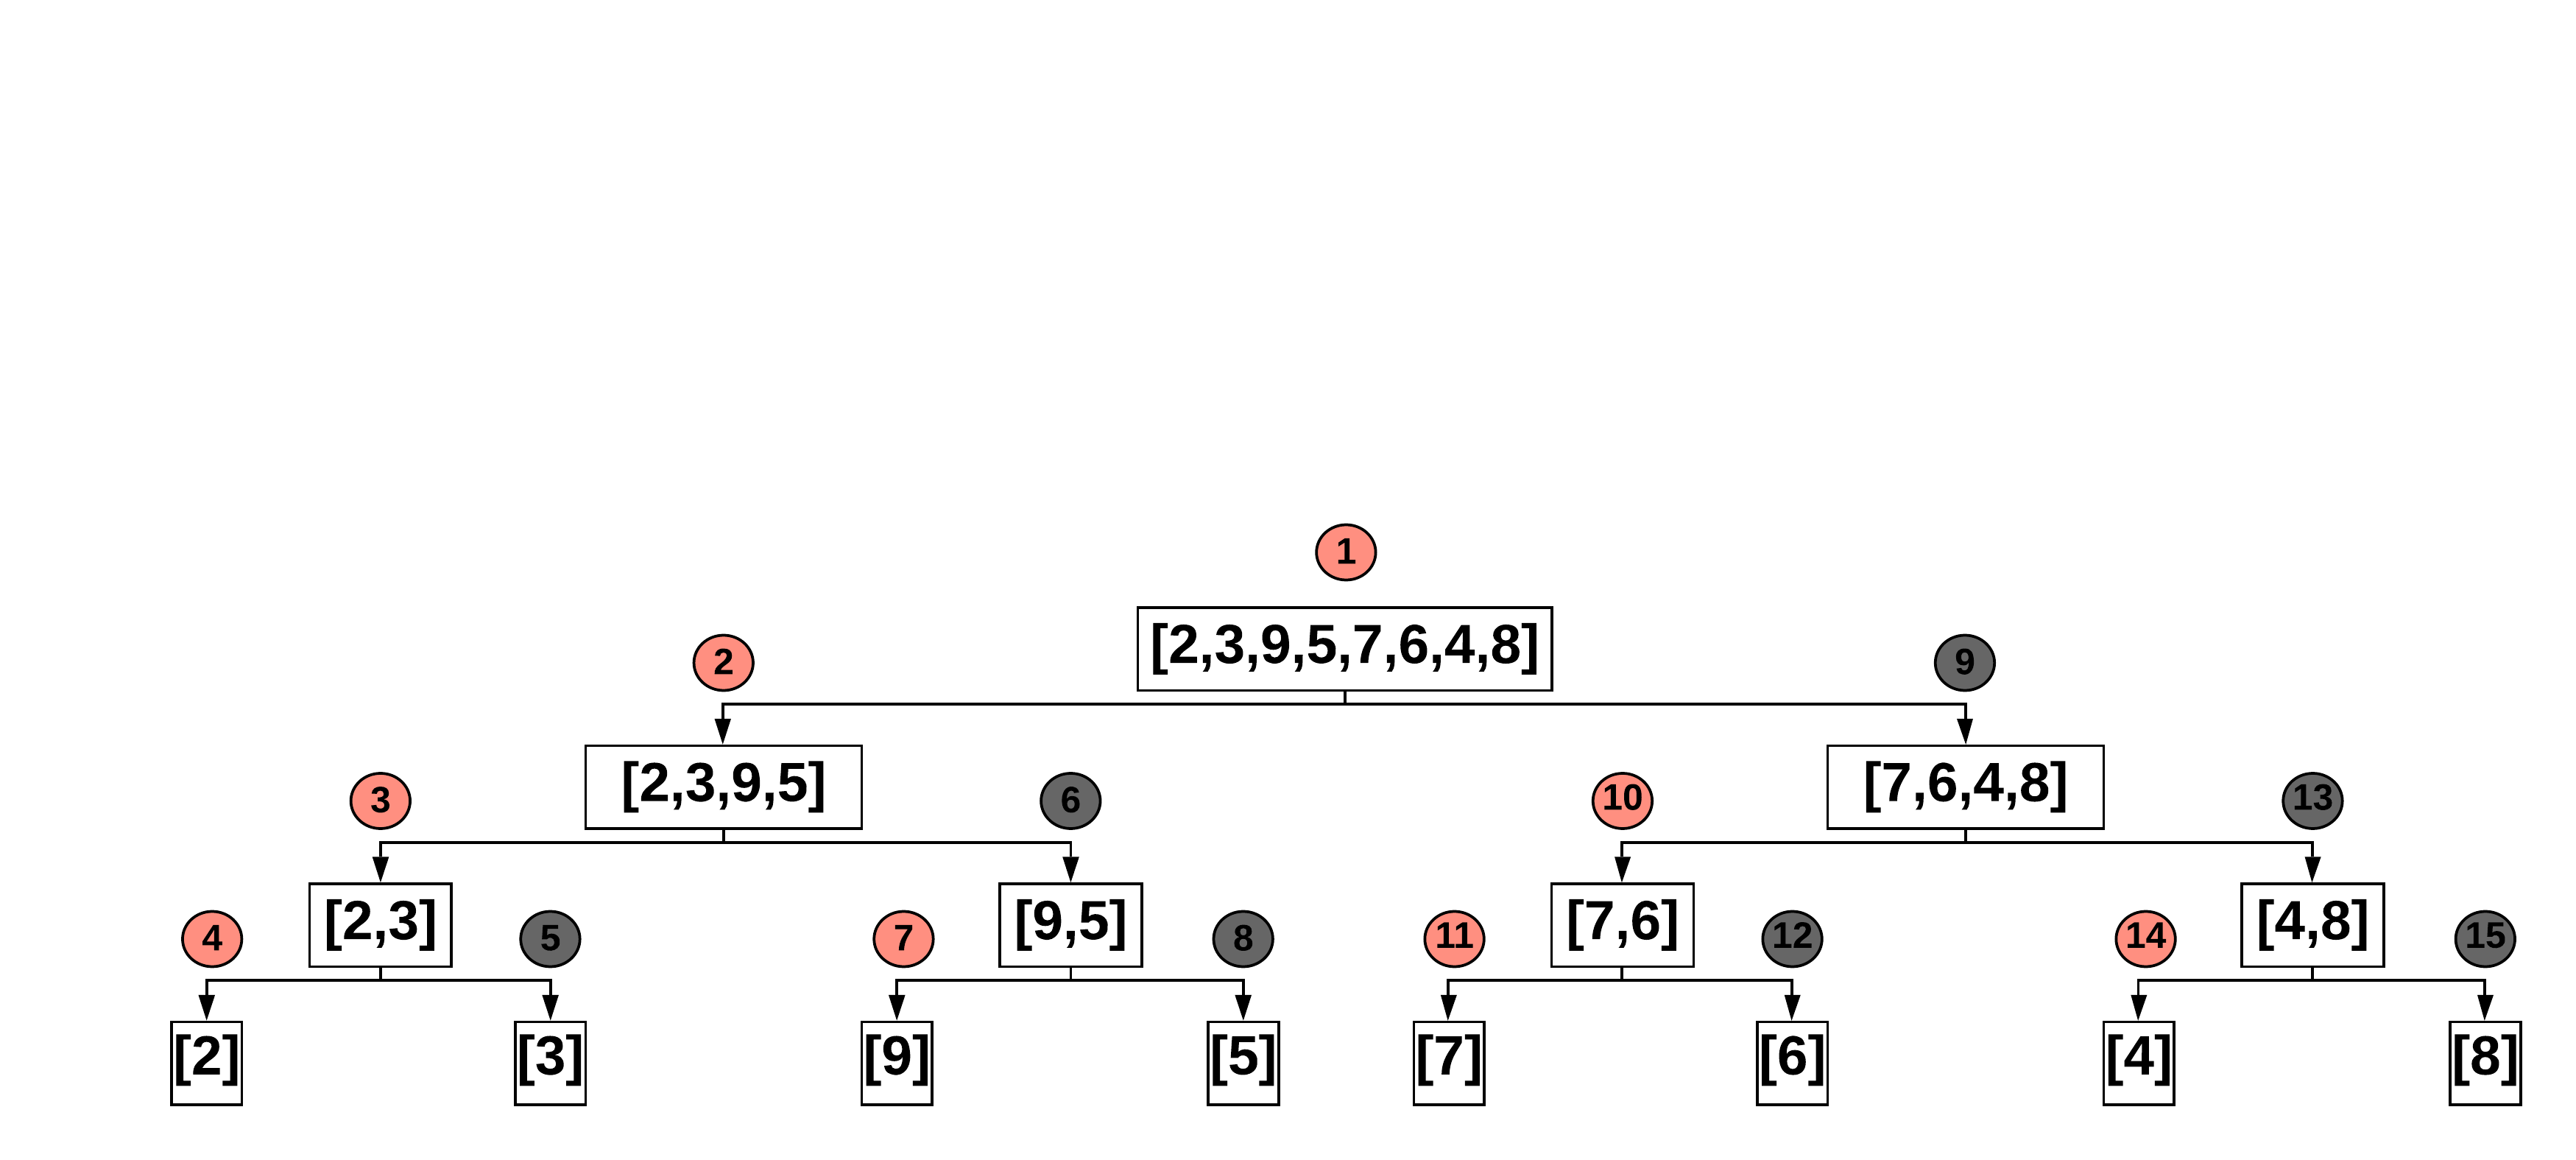
\includegraphics[scale=0.45]{mergesort_recursion.png} 
\caption{Schematic of the recursive sequence of calls made by the MergeSort algorithm to create sub-arrays when provided with the input array $A = [2,3,9,5,7,6,4,8]$. Each arrow denotes a recursive call with the exact sequence of calls denoted by the number in a each circle, and the elements of each recursive sub-array shown between square brackets. Red- and grey-shaded circles correspond to first and second recursive calls in the MergeSort algorithm shown in Listing \ref{mergeSortSource}. This diagram was generated by the author using Lucidchart \cite{lucidchart}.}
\label{mergeSortDiagram1}
\end{figure}



Secondly one should note the order, or sequence, of recursive calls. Whilst sub-arrays 1 and 8 appear to be called sequentially in Listing \ref{mergeSortSource}, the left-most tree is explored entirely until the base recursive condition is met, that is, when an array containing only one element is obtained. 

Figure \ref{mergeSortDiagram2} in turns shows the subsequent merging of arrays into a final sorted array. The merge operation occurs after the second recursive call to the MergeSort algorithm, lines $34-58$ of Listing \ref{mergeSortSource}. When merging arrays the left and right arrays are traversed at the same time and the element at index 1 in the first array is compared with the element at the same index in the second array. The lesser of the two elements is put into the sorted array first, followed by the other, and this process is repeated for all shared indices. 

In cases where there are two sub-arrays of unequal size, the elements in the larger array are added in sequence once the two sub-arrays have been compared, as shown in lines $47-58$ of Listing \ref{mergeSortSource}. Note therefore that one would expect a subtely different set of diagrams depending on the number of elements in the original array, and thus each sub-array, but the algorithmic and logical approaches are entirely self-similar and the algorithm shown in Listing \ref{mergeSortSource} is applicable to arrays of any number of elements -- heap space allowing.

\begin{figure}[t!]
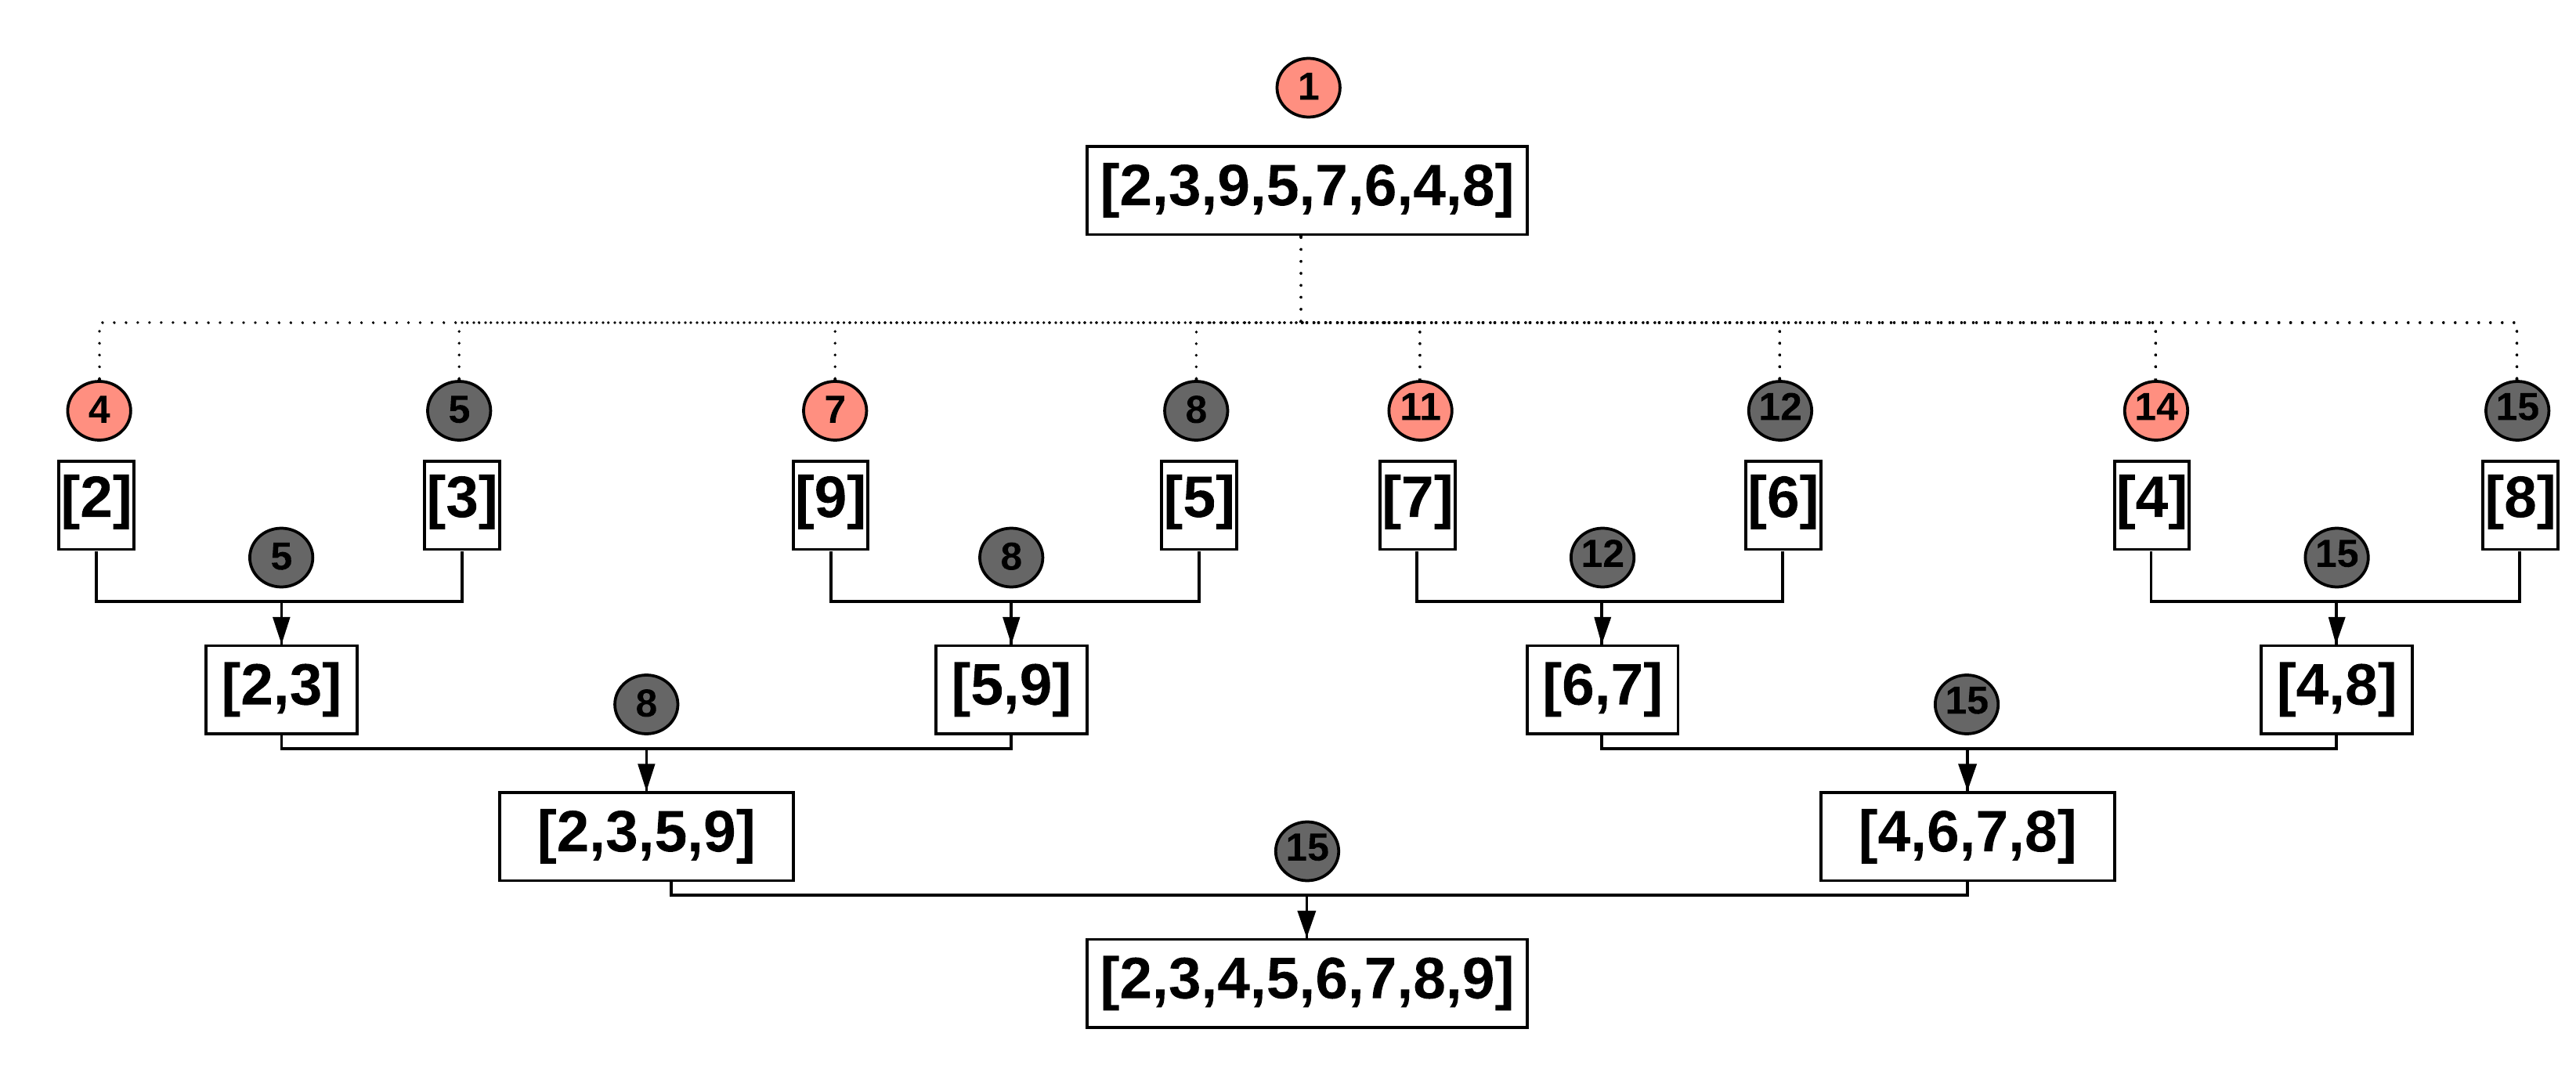
\includegraphics[scale=0.475]{mergesort_merge.png} 
\caption{Schematic of the sequence of merge operations made by the MergeSort algorithm when provided with the input array $A = [2,3,9,5,7,6,4,8]$. The corresponding recursive creation of sub-arrays is shown in Figure \ref{mergeSortDiagram1} along with a description of each symbol. Each arrow indicates the merging of two-subarrays into a sorted array, as shown algorithmically lines $34-58$ of Listing \ref{mergeSortSource}. This diagram was generated by the author using Lucidchart \cite{lucidchart}.}
\label{mergeSortDiagram2}
\end{figure}

In terms of time-complexity MergeSort is equivalent to QuickSort in the average- and best-case scenarios, with both displaying $\Theta(n \log n)$ and $\Omega(n \log n)$ performance. The initialiazation of the two sub-arrays from the $n$ elements in the base array is an $\Theta(n)$, $\Omega(n)$ and $\mathcal{O}$($n$) operation as all elements must be individually accessed during the loop. Similarly, the merge operations, shown as three individual $while$ loops in lines $34-58$ of Listing \ref{mergeSortSource} all have $\Theta(n)$, $\Omega(n)$ and $\mathcal{O}$($n$) time-complexity. 

The $\log n$ component of MergeSort's time-complexity stems from the recursive calls required to split the array of $n$ elements into $n$ arrays of 1 element, which requires $\approx \log(n)$ recursive calls. For each of the $\log(n)$ recursive calls, the $\mathcal{O}$($n$) operations described previously must be carried out and ignoring constant terms the asymptotic $\Theta(n \log n)$, $\Omega(n \log n)$ and $\mathcal{O}$($n$) behaviour is thus rationalised as the product of these two terms. 

As noted previously, unlike QuickSort, MergeSort does not rely on the selection of a pivot element about which the partitioning of sub-arrays is dependent and the poor worst-case $\mathcal{O}$($n^2$) performance of QuickSort is avoided entirely with MergeSort as a result of the consistently well-balanced left and right trees. However, this may not be reflected in overall performance, as will be shown and discussed in subsequent benchmarking studies. One reason for this is MergeSort's added requirements in terms of space. During each recursive call the $n$ array elements are first partitioned into and stored in two newly created arrays, requiring auxiliary storage which leads to $\mathcal{O}$($n$) space-complexity, versus $\approx \log n$ space-complexity in the case of QuickSort which can be implemented entirely in-place without large auxiliary memory.

\section{Implementation and Benchmarking}
\subsection{Java Application Overview}
The specific implementation of each algorithm being benchmarked has been described in the previous section and will not be elaborated upon here. This section will give a broader perspective on the main features of the Java application used to benchmark these algorithms. The Java application was developed with object-orientated programming principles in mind, that is, abstraction, encapsulation, cohesion, coupling, and composition. In this regard there are several packages in the final \textsc{Java} project -- \emph{runner}, \emph{sorters}, \emph{random}, and \emph{printers} which, in tandem, produce meaningful algorithm benchmarks and output which is useful for the user. Note that unlike the previous code Listings which provided complete details of each algorithm, the code Listings below are condensed in places, in some instances code has been removed for brevity, and the main aim is to give an indicative overview the various classes, methods and procedures implemented in the current project. Comprehensive detail of all packages, classes and methods are provided in the Java source code, and the accompanying JavaDocs, which have been compiled and included in the \emph{doc} directory of the project source code.

The package central to \emph{this} project is the \emph{sorters} package, which contains two classes. The first is \emph{sorters.AbstractSorter}, a minimalist abstract base class defining the methods expected of a concrete \emph{sorter} class -- a \emph{setSortMethod()}, a \emph{getSortMethod()}, and crucially, a \emph{sort()} method. The first and last methods give a good indication of the procedures used herein -- to sort an array a ``sorter'' type must be used, the ``setSortMethod'' must be called to define a specific algorithm to be used, and finally, the ``sort'' function should be called. The concrete \emph{sorters.IntegerSorter} class extends the \emph{sorters.AbstractSorter} abstract base class by implementing the aforementioned methods, and each sorting method implemented in the current project is present as an individual method in the \emph{sorters.IntegerSorter} class. 

Code Listing \ref{IntegerSorter} below provides a condensed overview of the \emph{IntegerSorter} class and its methods. The sort methods to be used can be set via the \emph{IntegerSorter.setSortMethod(String sortMethod)} method, where a single lowercase \emph{String} denotes the sort method to be used -- the options are:

\begin{itemize}
\item \emph{bubble} for BubbleSort
\item \emph{quick} for QuickSort
\item \emph{counting} for CountingSort
\item \emph{insertion} for InsertionSort
\item \emph{merge} for MergeSort
\item \emph{selection} for SelectionSort
\end{itemize}  

Note that although SelectionSort was not described previously, it has been implemented \cite{selection_sort} in Java and benchmarked as a result of the Author's curiosity with little extra burden in terms of application design or configuration.



\begin{lstlisting}[caption={An overview of the \emph{IntegerSorter} class and its methods.},captionpos=b, label={IntegerSorter}]
public class IntegerSorter extends AbstractSorter<int[]> {

	private String sortMethod;
	
	public IntegerSorter() {}
	
	public String getSortMethod() {}

	public void setSortMethod(String sortMethod) {}
	
	@Override
	public long sort(int[] input) {

		sortMethod = sortMethod.toLowerCase();
		long runTime = -1;

		if (sortMethod.equals("bubble")) {
			// start the timer
			long startTime = System.nanoTime(); 
			
			// run the sort
			IntegerSorter.iterativeBubbleSort(input); 
			
			// compute the CPU time in nanoseconds
			runTime = System.nanoTime() - startTime; 
		}
		else if (sortMethod.equals("quick")) {}
		else if (sortMethod.equals("counting")) {}
		else if (sortMethod.equals("merge")) {}
		else if (sortMethod.equals("insertion")) {}
		else if (sortMethod.equals("selection")) {}
		else {}
		
		// return the run time in nanoseconds
		return runTime;
	}	
	
	public static void iterativeBubbleSort(int[] array) {}
	public static void insertionSort(int[] array) {}
	public static void selectionSort(int[] array) {}
	public static void countingSort(int[] array) {}
	public static void mergeSort(int[] array) {}
	public static void quickSort(int[] array, int low, int high) {}
}
\end{lstlisting}

Once a sorting method has been chosen, arrays of integers can be sorted \emph{via} the \emph{IntegerSorter.sort(int[] input)} method, which will delegate the responsibility for sorting to a specific sort method. The \emph{IntegerSorter.sort(int[] input)} ultimately returns a \emph{long} type containing the benchmark CPU time in nanoseconds. 

Importantly with respect to all benchmark CPU times computed, the benchmark time includes only the call to a specific sort method, and a subsequent call to \emph{System.nanoTime()} -- no other methods (i.e. array generation), which might conflate or artificially inflate the CPU times, are called between the call to the sort method and the timer call. The computed benchmark CPU time are therefore wholly representative of the effiency of a given algorithm (as implemented), and these efficiencies are comparable between iterations of a single algorithm, and between different algorithms.

In order to run benchmarks and store benchmark times for a given algorithm, array size, and iteration, an \emph{AlgorithmBenchmarker} class has been developed and included in the \emph{runner} package. An \emph{AlgorithmBenchmarker} instance has responsibility for running benchmarks, and storing relevant information for a single algorithm and array size (i.e. a single ``cell'' in the output tables). However, it also stores information for \emph{multiple} statistical runs, thus allowing for summary statistics to be readily computed, stored and retrieved. The \emph{AlgorithmBenchmarker} class contains $\approx$ 20 methods in total, including \emph{Bean}-methods (getter/setters), not all of which will be described here. The most useful and pertinent classes relate to:

\begin{itemize}
	\item benchmarking an algorithm \emph{n} times \emph{via}:
	\begin{itemize}
		\item \emph{runIntegerBenchmark()}
	\end{itemize}
	\item computing statistical properties \emph{via}: 
	\begin{itemize}
		\item \emph{calculateMeanRunTime()}
		\item \emph{calculateStandardDeviation()}
		\item \emph{sampleStandardDeviation()}
		\item \emph{populationStandardDeviation()})
	\end{itemize}
	\item retrieving best, average and worse case run times \emph{via}:
		\begin{itemize}
		\item \emph{getMeanRunTime()}
		\item \emph{getBestRunTime()}
		\item \emph{getWorstRunTime()}
		\item \emph{getProperty()} (which retrieves info. from a data dictionary)
		\end{itemize}
\end{itemize}

Perhaps the most important method is the \emph{AlgorithmBenchmarker} class is the \emph{runIntegerBenchmark()} method, as outlined in Listing \ref{runIntegerBenchmark} below which provides an overview of some, but not all, of the source code. This method takes as input a) any type which extends an \emph{AbstractSorter} type, i.e. an \emph{IntegerSorter} b) a single integer defining the size of the array to be benchmarked, and c) a single integer defining the number of iterations to run. A loop is then initialized to run \emph{n} times, once for each iteration requested, and during each loop a new array of random integers of a specific size is generated via a call to the \emph{random.ArrayFactory.generateIntegers()} method, which will generate an array of random positive integers. An important point is that for every algorithm, array size, and iteration that is benchmarked, a new, unsorted, array of random integers is generated.

\begin{lstlisting}[caption={An overview of the \emph{runIntegerBenchmark()} method} in the \emph{AlgorithmBenchmarker} class.,captionpos=b, label={runIntegerBenchmark}]
public void runIntegerBenchmark(
							AbstractSorter<int[]> sorter, 
							int arraySize, int numberOfIterations
							) {

	// set the array size and samples per array size
	this.arraySize = arraySize;
	this.numberOfIterations = numberOfIterations;

	// benchmark the sorting algorithm numberOfIterations times
	for (int i = 0; i < this.numberOfIterations; i++) {

		// generate an array of random numbers of
		// a given size before each sorting operation
		int[] array = ArrayFactory.generateIntegers(arraySize);
		
		// run the sort method and store the runTime
		// in the AlgorithmBenchmarker.iterationData ArrayList
		long runTime = sorter.sort(array);
		this.iterationData.add(runTime);
	}	
}
\end{lstlisting}

The \emph{IntegerSorter} class coupled with the \emph{AlgorithmBenchmarker} class therefore allow benchmarks to be carried out for multiple sort algorithms, multiple array sizes, and for multiple iterations in a reasonably straight forward manner \emph{via} the \emph{Runner.runIntegerSortBenchmarks()} method. Listing \ref{runIntegerSortBenchmarks} below provides an overview of the general approach. 

\clearpage

\begin{lstlisting}[caption={An overview of the \emph{runIntegerSortBenchmarks()} method} in the \emph{Runner} class.,captionpos=b, label={runIntegerSortBenchmarks}]
private static ArrayList<AlgorithmBenchmarker> runIntegerSortBenchmarks(
		int[] arraySizes, 
		int samplesPerArraySize,
		String[] algorithms) {
	
	// create a single integer sorter instance
	// to be used to call various sort methods
	IntegerSorter integerSorter = new IntegerSorter();

	// a list to store all the AlgorithmBenchmarker instances
	// which will run benchmarks and store results
	ArrayList<AlgorithmBenchmarker> algorithmBenchmarkers = new ArrayList<AlgorithmBenchmarker>();

	// for each algorithm ...
	for (String algorithm : algorithms) {

		// set the sort method
		integerSorter.setSortMethod(algorithm);

		// for each array size ... i.e. 100 elements, 200 elements
		for (int arraySize : arraySizes) {
			
			// create a new AlgorithmBenchmarker instance
			// to run the benchmarks
			AlgorithmBenchmarker benchmarker = new AlgorithmBenchmarker(algorithm);
			algorithmBenchmarkers.add(benchmarker);

			// run the benchmark by providing the 
			// integerSorter instance, the array size
			// to be benchmarked and the number of
			// times to run the benchmark
			benchmarker.runIntegerBenchmark(integerSorter, arraySize, samplesPerArraySize);					
		}
	}

	// return the list of algorithm benchmarkers
	return algorithmBenchmarkers;
}
\end{lstlisting}

\clearpage

The \emph{runIntegerSortBenchmarks()} takes as input an array of integers (\emph{arraySizes}) specifying the array sizes to be benchmarked (i.e. 100 elements, 200 elements, etc), an integer defining the number of samples to be run for each array size (\emph{samplesPerArraySize}), and a \emph{String} array containing the names of the various sorting methods to benchmark (\emph{algorithms}). 

For each algorithm, and for each array size the benchmark is then run \emph{n} times with the results stored in a specific \emph{AlgorithmBenchmarker} instance. Each instance of the latter is added to an \emph{ArrayList} of \emph{AlgorithmBenchmarker} instances, each of which can be later retrieved and used for data analysis.

The above approach outlines how sorting benchmarks can be carried out in batches of arbitrary size and complexity -- that is, multiple algorithms, multiple array sizes, and multiple iterations per array size. These procedures are initiated from the \emph{Runner} class \emph{via} its \emph{main} method as shown in Listing \ref{main} below.

\begin{lstlisting}[caption={An overview of the \emph{main()} method} in the \emph{Runner} class.,captionpos=b, label={main}]
public static void main(String[] args) {

	// get the list of algorithms to run
	String[] algorithms = Runner.getAlgorithmsToRun();
	
	// define the number of samples to be run for
	// each algorithm/array size
	int samplesPerArraySize = 10;

	// generate a list of sample sizes, n, 
	// which determine the number of elements
	// in an array to be sorted
	int[] arraySizes = Runner.generateArraySizes(100, 20);

	// run a batch of integer sort benchmarks
	ArrayList<AlgorithmBenchmarker> algorithmBenchmarkers;
	algorithmBenchmarkers = Runner.runIntegerSortBenchmarks(arraySizes, samplesPerArraySize, algorithms);

	// print the output data by delegation to the 
	// printers.BenchmarkDataPrinter class
	Runner.printOutputData(algorithms, arraySizes, samplesPerArraySize, algorithmBenchmarkers);

}
\end{lstlisting}

Firstly a list of algorithms are generated \emph{via} a call to the \emph{getAlgorithmsToRun()} method in the \emph{Runner} class. The number of iterations to run for each sorting benchmark is subsequently defined. 

Next an array of integers corresponding to the array sizes which will be sorted is generated \emph{via} a call to the \emph{generateArraySizes()} method in the \emph{Runner} class. The array sizes are generated by provided the lower bound to the number of array elements (100 elements in the Listing \ref{main} above). This lower bound is increased in multiples of two \emph{n} times, where \emph{n} is defined as 20 on line 13 of Listing \ref{main} above. Note that this exponential increase in array sizes will quickly lead to some inefficient algorithms taking undesirable lengths of time to complete the sorting procedure. For this reason, specific upper bounds to array sizes for all algorithms have been specified in the \emph{getAlgorithmSpecificMaxArraySizes()} method. 

For inefficient comparison based sort algorithms, this upper bound is set to $\approx$ 60,000 elements. For the most efficient algorithms arrays containing over 1 $\times$ 10${^8}$ elements could be sorted on reasonable timescales. Although not shown in Listing \ref{runIntegerSortBenchmarks}, which gives an overview of how batches of benchmarks are run, these restrictions on whether a specific array size will be benchmarked for a specific algorithm are enforced therein, in the \emph{runIntegerSortBenchmarks()} method in the \emph{Runner} class.

Once the algorithms to be benchmarked are defined, the number of iterations for each array size are set, and the list of array sizes to run have been initialized, the benmchmarking procedure is initiated \emph{via} a call to the \emph{runIntegerSortBenchmarks()} method in the \emph{Runner} class, line 17 of Listing \ref{main}.

Finally, the list of \emph{AlgorithmBenchmarker} instances returned from the benchmarking runs are passed to the \emph{printOutputData()} method of the \emph{Runner} class, along with the list of algorithms, array sizes etc. The \emph{printOutputData()} method delegates responsibility for producing neatly-formatted output to the \emph{BenchmarkDataPrinter} class in the \emph{printers} package.

The \emph{BenchmarkDataPrinter} class contains a number of useful print methods which will be briefly described but source code will not be discussed in detail. The \emph{printBenchmarkPropertyToScreen()} method prints various benchmark results to the terminal or console that one runs the code in - it is useful for quick inspection of results. The \emph{printBenchmarkPropertyToFile} and \emph{printIterationDateToFiles()} write similar outputs to files. The \emph{printBenchmarkPropertyToFile()} method produces tabular output in multiple files in the \emph{./summary\textunderscore data} directory, which will be created in whatever directory the source code is called from. Similarly the \emph{printIterationDateToFiles()} prints iteration-specific benchmark CPU times to files in the \emph{./iteration\textunderscore data} directory, which will also be created if it does not exist.

For each algorithm and array size, the benchmark properties are computed over \emph{n} iterations, and the outputs printed to the screen and to disk include:

\begin{itemize}
	\item the mean run time ($\mu$)
	\item the best-case run time
	\item the worst-case run time
	\item the variation in run times ($\sigma$)
	\item the coefficient of variation in run times as a \% ( $100\times \sigma / \mu$)

\end{itemize}

The mean simulation time, $\mu$ is given by 

\begin{equation}
\mu = \frac{1}{n}\sum_{i=1}^{n}t_i 
\end{equation}

where $t_i$ is the time taken to complete a single array sort, and $n$ is the total number of sorts performed. The variation, $\sigma$ is given by:

\begin{equation}
\sigma = \sqrt{\frac{1}{n-1}\sum_{i=1}^{n}(t_i-\mu)^2}
\end{equation}

when $n \leq$ 100, and:

\begin{equation}
\sigma = \sqrt{\frac{1}{n}\sum_{i=1}^{n}(t_i-\mu)^2}
\end{equation}

when $n >$ 100, corresponding to sample and population standard deviations respectively. Irrespective of how $\sigma$ is computed, the final variations in benchmark times for a given algorithm and array size are reported as 2$\sigma$ uncertainties, thus representing a $\approx$ 95\% confidence interval.

In terms of visualisation of results, the tabular data written to file were designed to be compatible with the \textsc{Pandas} library of \textsc{Python}, with subsequent data visualisation and analysis carried out using the \textsc{Matplotlib} library. All benchmark data presented in the next section, and the corresponding python files, are provided in the \emph{./results\_plotters} directory.

Whilst specific CPU times are presented with units of time (nanoseconds internally, milliseconds when written to file and plotted below), one should note that CPU times vary depending on the specific hardware employed and other system usage settings (e.g. availability of memory for recursive algorithms, garbage collection). All computations were carried out on a quad-core 8$^{th}$ generation \textsc{Intel}\textregistered \ \textsc{Core} \texttrademark \ i5-8250U with a clock frequency of 1.60 GHz -- a modest performance chip given current standards. The L1, L2 and L3 caches are 32 kb, 256 kb, and 6144 kb. Whilst noting the CPU specifications is done for thoroughness, algorithms will ultimately be compared in terms of their $\mathcal{O}$($n$) notation and relative CPU times, and absolute CPU times are therefore of lesser importance.

Finally, the \textsc{Eclipse} integrated development environment (IDE) was used for code development and testing with the following Java environments: 
\begin{itemize}
\item openjdk 11.0.6 2020-01-14
\item  OpenJDK Runtime Environment \\(build 11.0.6+10-post-Ubuntu-1ubuntu118.04.1)
\item OpenJDK 64-Bit Server VM \\(build 11.0.6+10-post-Ubuntu-1ubuntu118.04.1, mixed mode, sharing)
\end{itemize}

The application as provided is configured to regenerate the results reported in Section 3.2. The total time to run those benchmarks is approximately 600 seconds. For faster tests one should probably modify the largest array size to be sorted by changing line 13 of the \emph{Runner.main()} method as shown in Listing \ref{main}, and re-compile the source code.

To run the Java code provided the following command suffices in a linux shell:

\begin{lstlisting}[caption={Calling the default JRE to run the algorithm benchmarks}.,captionpos=b, label={running1}]
	$ cd code/sort_benchmarks/bin/
	$ java runner.Runner
\end{lstlisting}

\begin{lstlisting}[caption={Calling a specific JRE to run the algorithm benchmarks} class.,captionpos=b, label={running2}]
	$ cd code/sort_benchmarks/bin/
	$ /usr/lib/jvm/java-11-openjdk-amd64/bin/java runner.Runner
\end{lstlisting}

If errors are encountered they are likely related to trying to run the code using a different version of Java than that used to compile the source. The quickest solution is to recompile the source code using a local Java compiler. Example terminal output is given in Listings \ref{terminalOutput1} and Figure \ref{terminalOutput2} below. Note that the timings therein are illustrative only and were produced during developmental testing.

\clearpage

\begin{lstlisting}[caption={Example terminal output from running the runner.Runner() method.},captionpos=b, label={terminalOutput1}]
--------------------------------------------------
-Runner.main()
--------------------------------------------------
--------------------------------------------------
-Runner.getAlgorithmsToRun()
--------------------------------------------------
-Will run the following algorithms:
	-bubble
	-insertion
	-selection
	-quick
	-counting
	-merge
--------------------------------------------------
--------------------------------------------------
-Runner.generateArraySizes()
--------------------------------------------------
-Run each algorithm for 20 different array sizes
	-Smallest array size = 100 elements
	-Largest array size = 52428800 elements
--------------------------------------------------
---------------------------------------------------------------
-Runner.runIntegerSortBenchmarks()
---------------------------------------------------------------
	-For each array size, and each algorithm run 10
	-samples to generate statistics on performance
---------------------------------------------------------------
--------------------------------------------------
-Runner.getAlgorithmsMaxArraySizes()
--------------------------------------------------
	-----------------------------------------------------------
	-Running [bubble] sort for array size of [100] integers
	-----------------------------------------------------------
	-mean  run time (nanoseconds)                     = 319351
	-best  run time (nanoseconds)                     = 279584
	-worst run time (nanoseconds)                     = 371549
	-variation in run time [+- 2.sigma] (nanoseconds) = 63720
	-variation in run time [+- 2.sigma] (% of mean)   = 19%
\end{lstlisting}

\clearpage

\begin{figure}
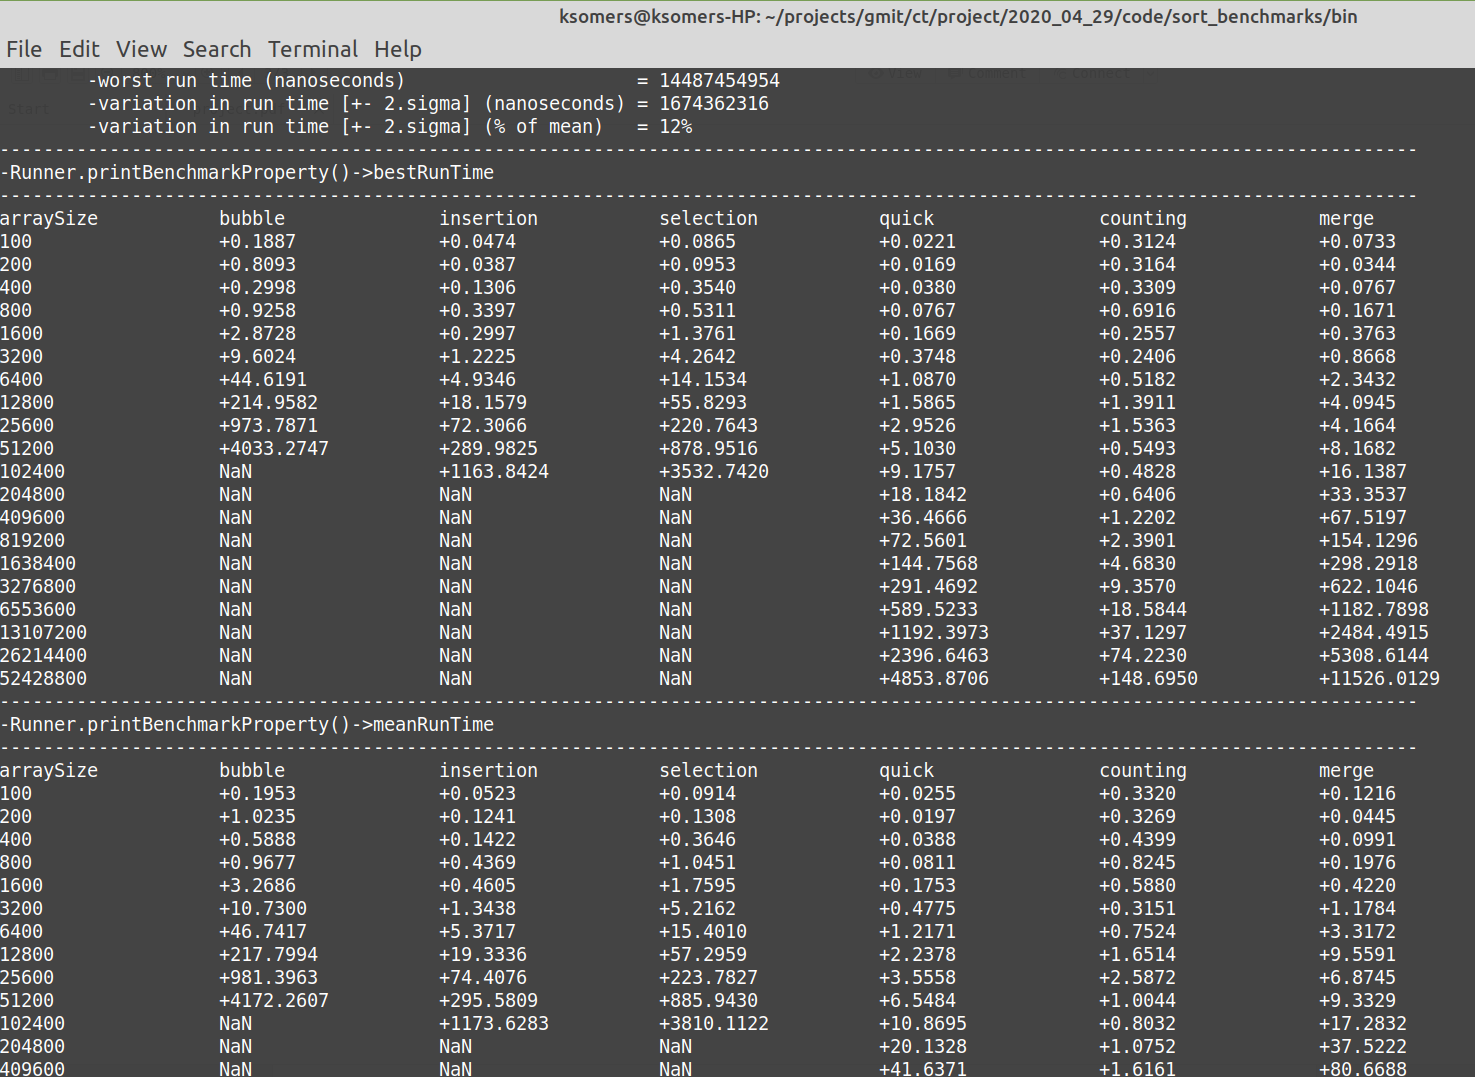
\includegraphics[scale=0.25]{screenshot.png} 
\caption{An illustrative screenshot of CPU times in milliseconds (best run time, mean run time) being written to a terminal for different algorithms and array sizes. $NaN$ values correspond to algorithms which were not benchmarked for a particular array size owing to their inefficiency.}
\label{terminalOutput2}
\end{figure}



\subsection{Benchmarking Results}
This section will describe and analyse the benchmarking results obtained from the algorithms described and implemented in previous sections. The specifics of each algorithm will not be re-iterated in detail as they have been described comprehensively in previous sections, and important conclusions from previous sections will merely be referred to when appropriate. The focus of this section will be to interpret the benchmarking results in terms of the theoretical characteristics of the  algorithms previously presented. Figure \ref{benchmark} and Table \ref{benchmarkTable} present the key results -- mean CPU times as a function of array size for each algorithm, each averaged over 10 samples.  Given the integer arrays being sorted are randomly distributed, it is safe to assume average-case $\Theta$ time-complexities when comparing algorithms.

\begin{figure}[t!]
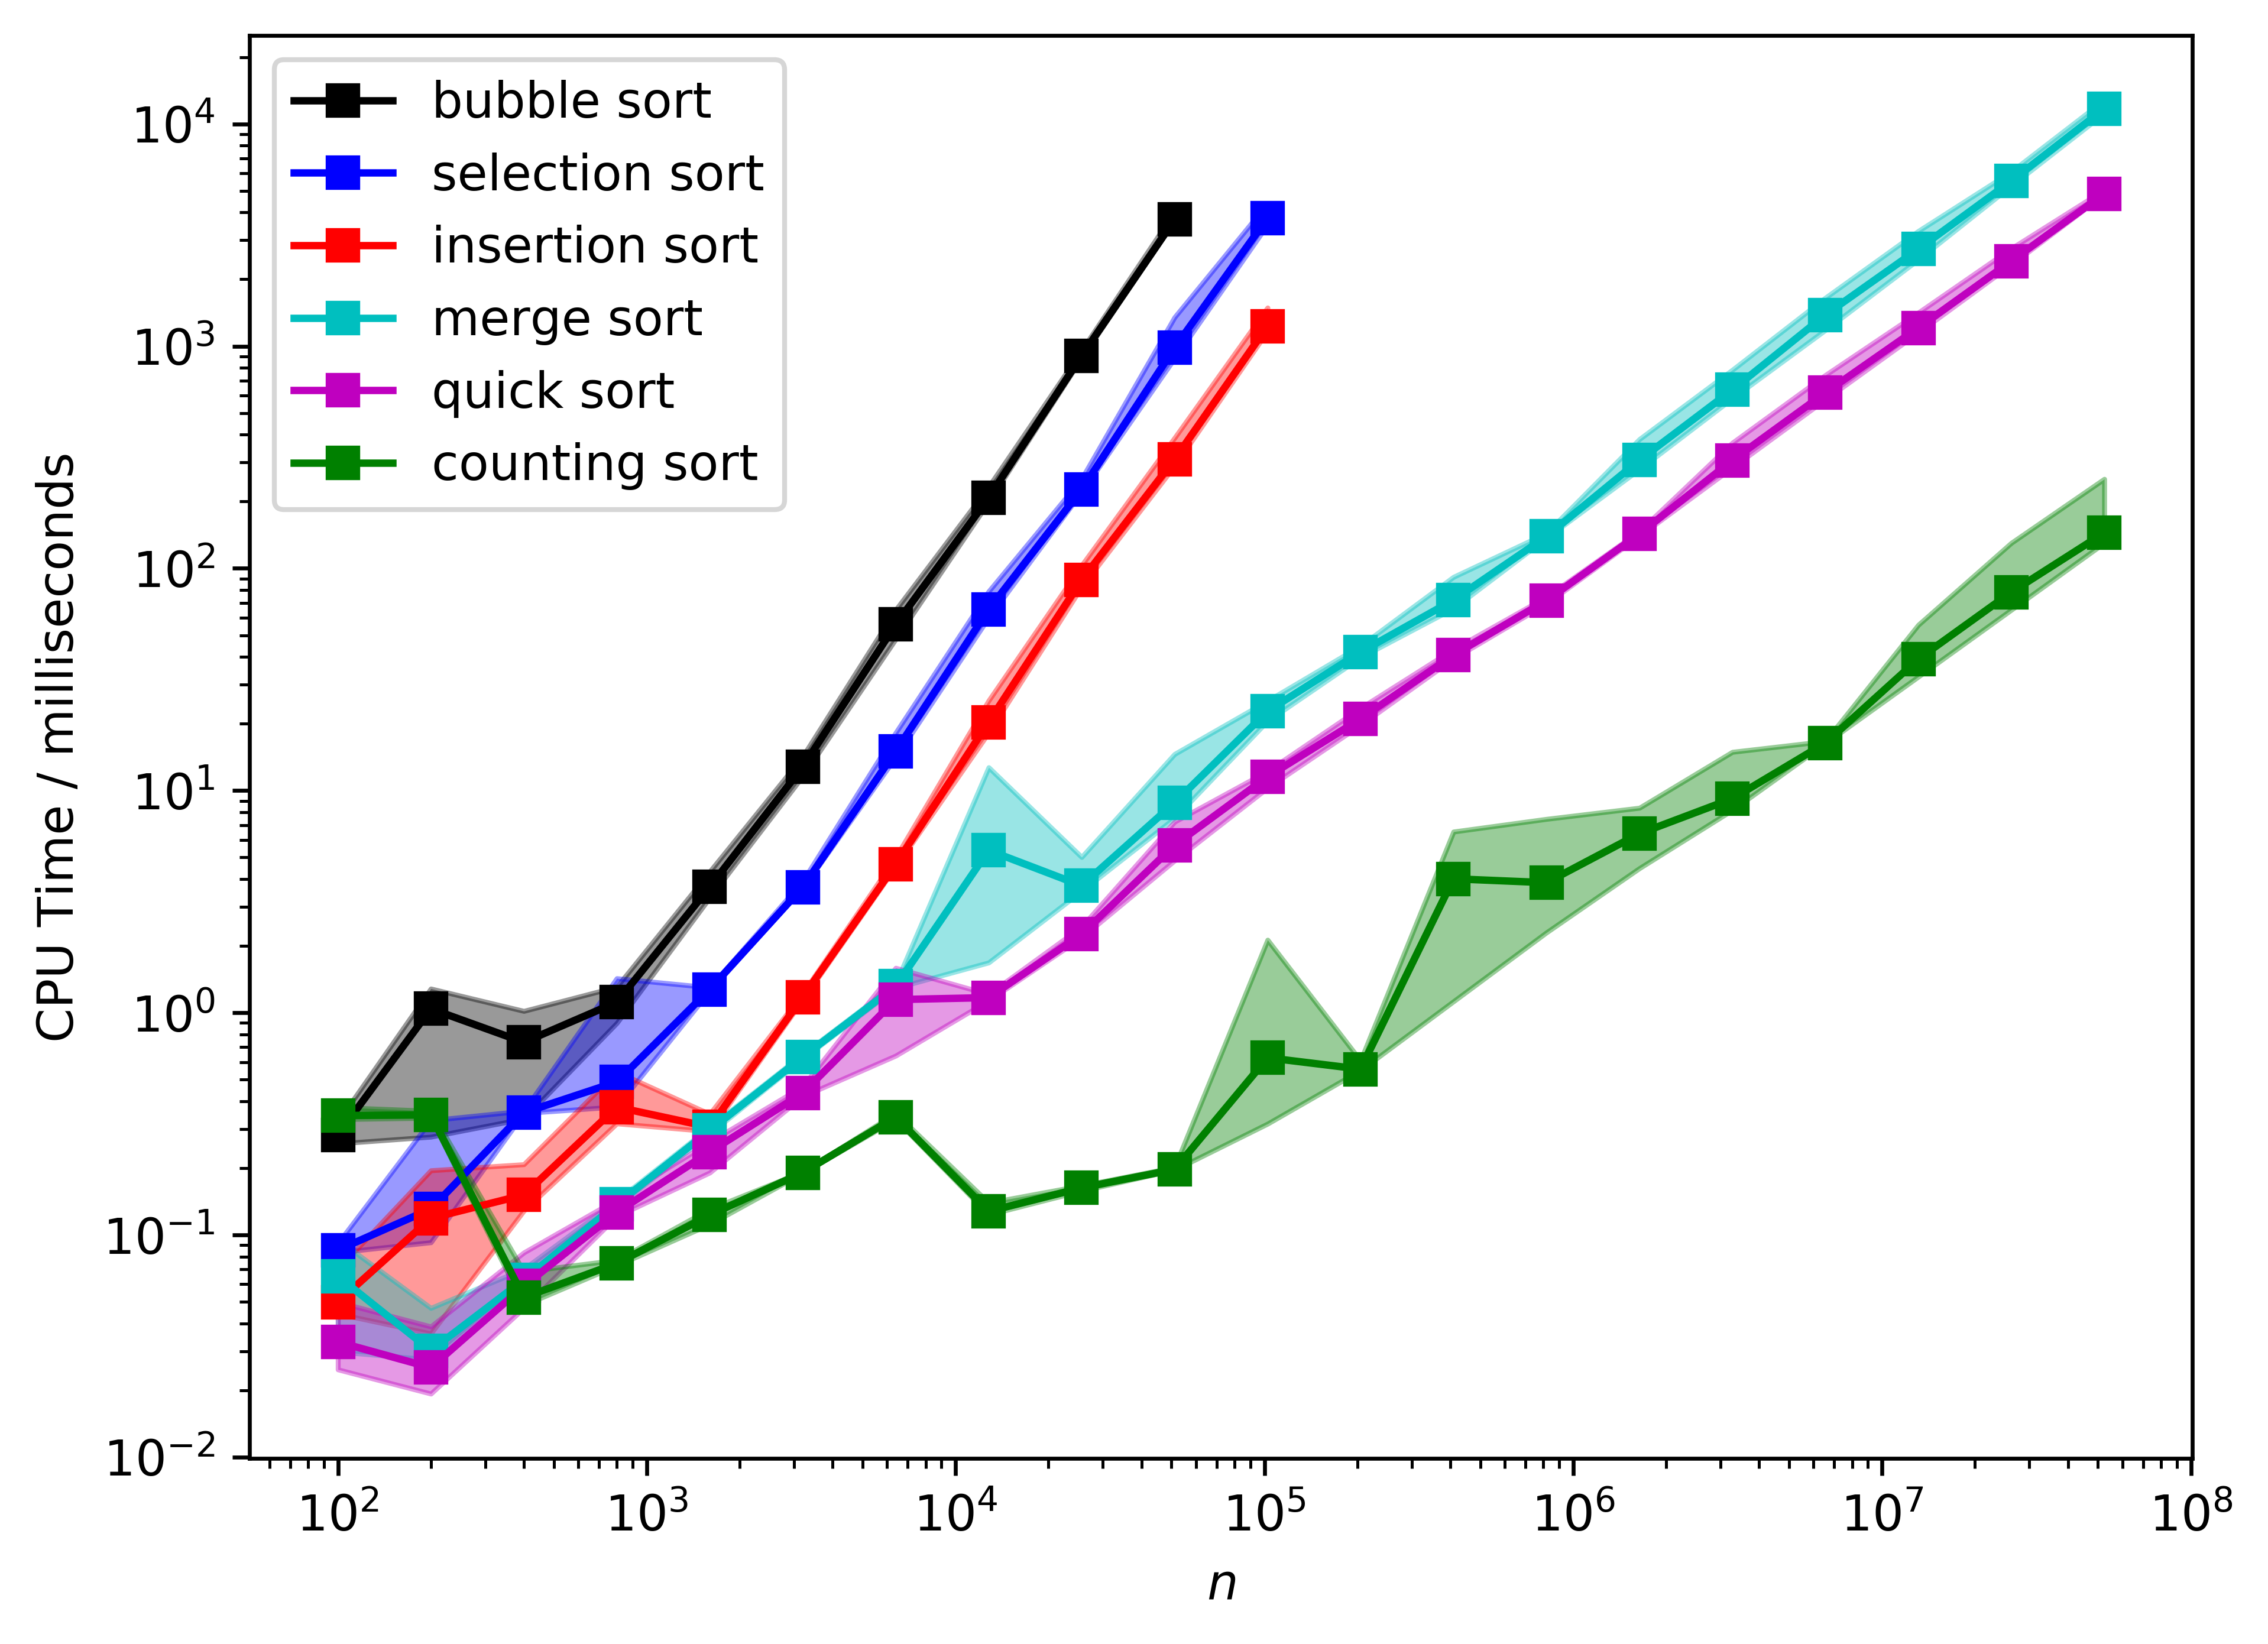
\includegraphics[scale=0.85]{benchmark_times_vs_nsamples_log_log.png} 
\caption{Benchmarking results obtained from the algorithms implemented in the current work where the $y$-axis is the CPU time in milliseconds, and the $x$-axis, $n$, is the number of elements in a given array. Lines and symbols represent the mean CPU time computed over 10 iterations for each algorithm and array size. The shaded regions represent the upper (worst-case) and lower (best-case) limits of the CPU times determined over 10 iterations. Both the $x$ and $y$ axes are represent on logarithmic scales.}
\label{benchmark}
\end{figure}


In Figure \ref{benchmark} each symbol corresponds to the mean CPU time, with corresponding shaded regions indicating the bounds for the largest (worst-case) and smallest (best-case) sorting times for a given array size $n$. One should note therefore that there are fluctations between CPU times computed for a given algorithm/array size but the general trends are still sensible, different algorithms can be compared and differentiated with certainty, and the fluctuations are generally modest for large values of $n$ which are of most interest. It is also worth stating that Figure \ref{benchmark} presents the benchmark results on a $\log$-$\log$ scale in order to emphasise similarities and differences more clearly, and so that different asymptotic behaviours, as implied by the slope of each line, can be clearly observed for algorithms with different time-complexity.

The three simple comparison-based sorts, BubbleSort, InsertionSort, and SelectionSort (which is included in the benchmarks for comparative and illustrative purposes \cite{selection_sort}, but not described in detail previously) all have theoretical average-case time-complexity of $\Theta(n^2)$. Figure \ref{benchmark} clearly shows they have same asymptotic behaviour with all methods having the same slope. 

BubbleSort consistently shows the worst overall performance for any appreciable value of $n$. Note that the BubbleSort algorithm implemented herein was modified, as shown in Listing \ref{bubbleSortSource2}, to account for scenarios where no inversions are required, a modification which was not introduced to other algorithms. Developmental testing showed that this modification had only a modest influence on the absolute CPU times, and no effect on the apparent asymptotic behaviour for large values of $n$. Despite the fact that InsertionSort and SelectionSort have better absolute performance than BubbleSort, which makes them objectively better sorting algorithms from an efficiency perspective, they all follow the same behaviour as $n$ tends to infinity, which effectively rules all three out as effective sorting algorithms for all but the smallest arrays/lists.

QuickSort and MergeSort should also be analysed in tandem, given that they are both recursive comparison-based methods with $\Theta(n \log n)$ time-complexity, with both methods clearly showing the same behaviour in terms of the dependency of CPU times on array size. Notably, their asymptotic behaviour is markedely different from the previous algorithms which have $n^2$ time-complexity, and both algorithms can be employed to sort arrays orders-of-magnitude greater in size than the $n^2$ algorithms. 

QuickSort tends to outperform MergeSort by $\approx$ a factor of 2 in terms of absolute CPU times, although the differences tend to become greater as $n$ increases -- for arrays of $\approx 1 \times 10^5$ elements MergeSort is a factor of 1.9 times slower than QuickSort, this ratio increasing to a factor of 2.4 for the largest array of $\approx 5\times10^7$ elements. The likely reason is the greater space-complexity of MergeSort relative to QuickSort. QuickSort carries out sorting in-place, requiring a small amount of fixed auxiliary memory to store variables during each recursive call, and $\log n$ space-complexity is the norm. Conversely, MergeSort has $\mathcal{O}(n)$ space-complexity, requiring extra memory to store array elements in two newly created sub-arrays during each recursive call. Added to this is the time required to build these arrays, and the subsequent merging operations, both of which are $\mathcal{O}(n)$ operations, although the constant multipliers representing the number of $\mathcal{O}(n)$ operations is omitted in asymptotic analysis.

Whilst QuickSort outperforms MergeSort in the present case, which is effectively representative of average-case performance given that the arrays are randomly distributed, one should note the caveats discussed in Sections 2.3 and 2.6 related to pivot selection. MergeSort is guaranteed to have $n\log n$ time-complexity in the worst-, average- and best-cases owing to the well balanced binary trees which result upon recursion. Whilst QuickSort has the same performance in the average and best cases, its worst-case $\mathcal{O}(n^2)$ behaviour when pivot selection is poor should be considered, and MergeSort may outperform QuickSort in certain circumstances and may well be chosen in practice.

What is clear from the present analysis is that both QuickSort and MergeSort are superior to the simple comparison-based sorts, in terms of time-efficiency, for arrays greater than $10^3$ elements. For small arrays containing  $n<10^3$ elements, or situations where memory is an issue, InsertionSort may still be of use, as it has comparable efficiency to the recursive methods for small arrays, but it has the added benefits of being simple to implement, and has $\mathcal{O}(1)$ space-complexity.

Finally we consider the performance of the only non-comparison-based method implemented in the current project -- CountingSort. Figure \ref{benchmark} shows that it outperforms all other methods for arrays of size $n\geq1\times10^3$ elements. Its theoretical time-complexity is given by $\mathcal{O}(n+k)$, $\Theta(n+k)$ and $\Omega(n+k)$ in the worst-, average-, and best-case scenarios, where $n$ is the array size and $k$ is the range of discrete values between the minimum and maximum values in the array.

Given that the time-complexity of CountingSort is dependent on both the number of elements $n$, and the range of these elements, $k$, the results presented in Figure \ref{benchmark} neither account for nor give insight into the influence of $k$ on its performance. Therefore, an important detail which must be considered when considering its performance as presented in Figure \ref{benchmark} is the upper limiting value which could be assigned to any single integer during random array generation. For all algorithms, array sizes and iterations the randomly generate integer arrays were allowed to contain any integer in the range $0-100000$. As the arrays used for benchmarking were generated randomly from values in this range, the absolute value for $k$ is not known precisely for each array size $n$, and each iteration, when CountingSort was implemented.  

\begin{figure}[t!]
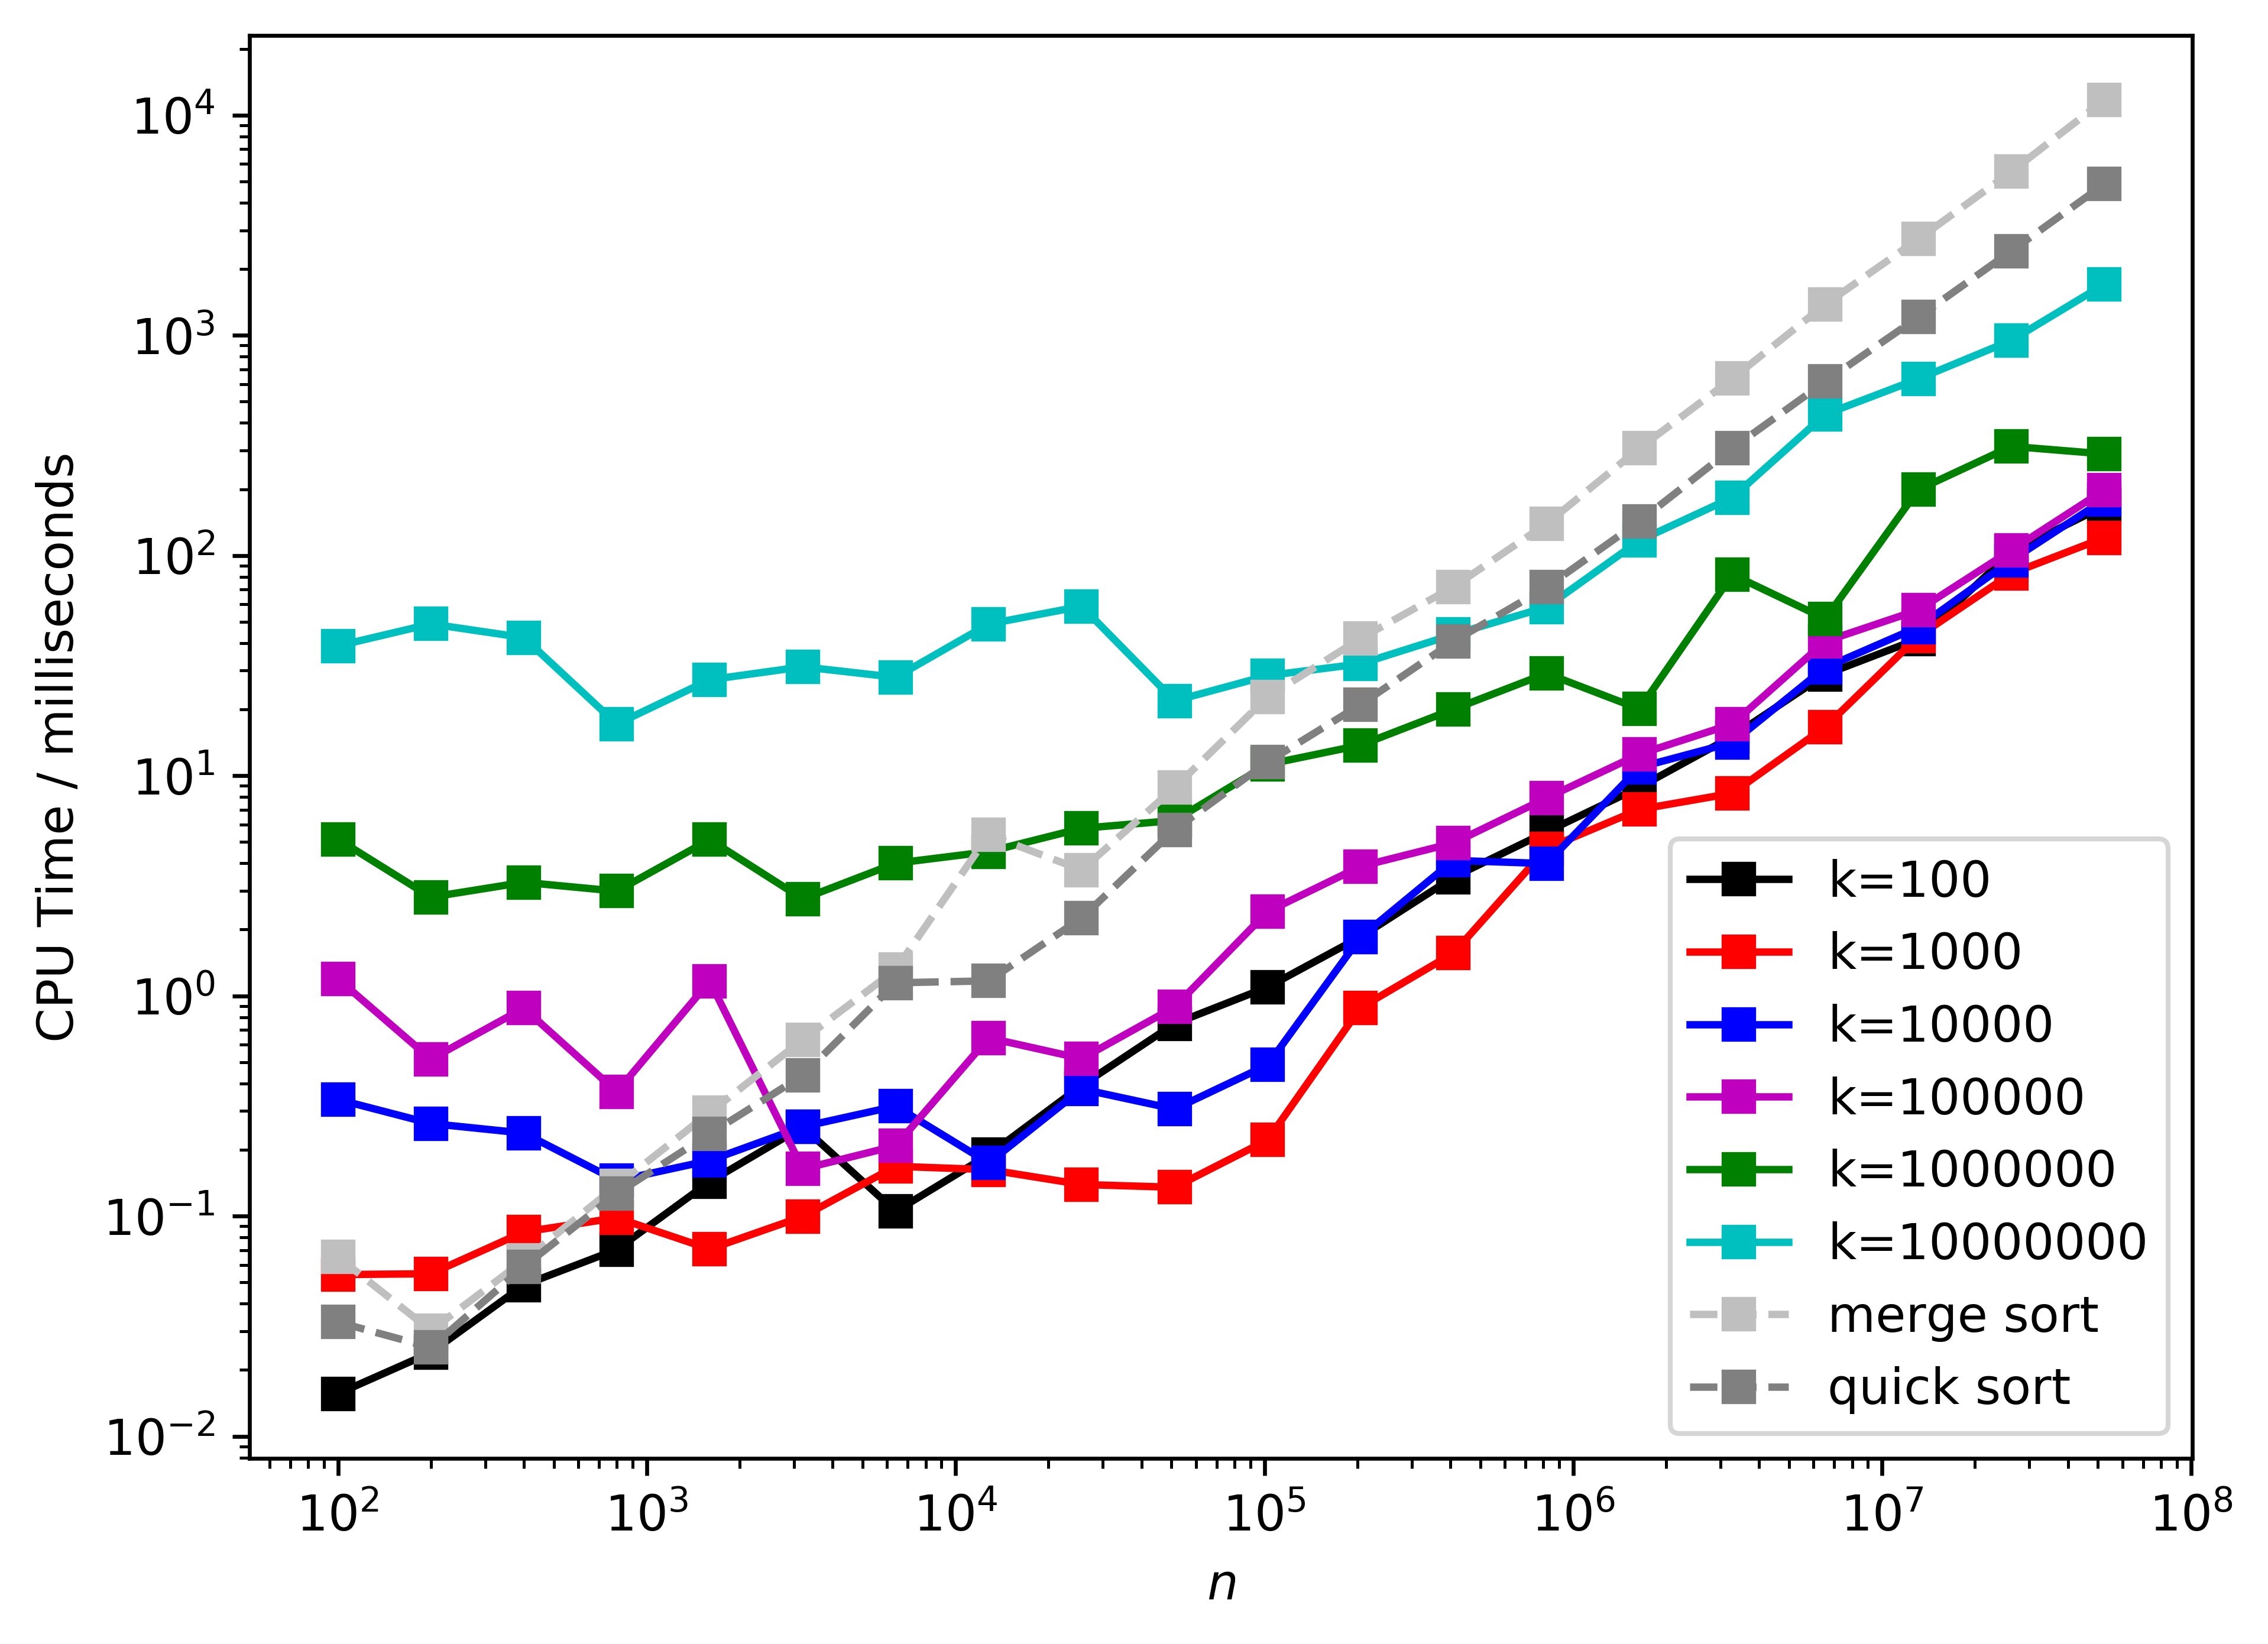
\includegraphics[scale=0.85]{counting_sort_n_k_data_log_log.png} 
\caption{Benchmarking results obtained from the CountingSort algorithm implemented in the current work where the $y$-axis is the CPU time in milliseconds, and the $x$-axis, $n$, is the number of elements in a given array. Lines and symbols represent the mean CPU time computed over 10 iterations for each algorithm and array size. Each series corresponds to simulation results where the range of integers in each array has been specficially set to the value indicated by $k$. Results from MergeSort and QuickSort from Figure \ref{benchmark} are included for comparitive purposes. Both the $x$ and $y$ axes are represent on logarithmic scales.}
\label{benchmark2}
\end{figure}


In order to get a better sense of the influence of $k$ on the performance of CountingSort, further simulations were run using CountingSort for various array sizes $n$, and fixed values of $k$. For these simulations $k$ was fixed by first generating an array of $n$ random integers, and subsequently defining two elements to be equal to 0 and $k-1$. 

Figure \ref{benchmark2} subsequently shows the combined influence of both $n$ and $k$, with $k$ clearly influencing the absolute CPU times for a given $n$. As expected, when $n<<k$ the efficiency of the algorithm is dominated by the $k$ term, as reflected by the near constant CPU times for a given $k$ when $k \geq 1\times10^4$ and $100 \geq n \leq 1\times10^3$. Conversely, where $n>>k$ the $n$ term is dominant, as illustrated for simulations where $n \geq 1\times10^6$ and $100 \geq k \leq 1\times10^5$. The intermediate case where $n\approx k$ results in the effiency being governed by some function $\propto n+k$ and both terms contribute to performance.

When considering the superior performance of CountingSort for large values of $n$ in Figure \ref{benchmark}, one should therefore be mindful of the caveat that $k$ is restricted to values no greater than $1\times10^5$. Indeed both MergeSort and QuickSort are shown to outperform CountingSort under certain conditions in Figure \ref{benchmark2}, and although not shown, BubbleSort, InsertionSort and SelectionSort may well outperform CountingSort where $n < 1\times10^3$ and $k > 1\times10^4-1\times10^5$.

To summarise, this report aimed to benchmark a number of comparison and non-comparison based sorting algorithms largely in terms of their time- and space-complexities. A number of popular sorting algorithms have been implemented in Java, and analysed from a theoretical perspective in order to understand their limiting behaviours, and to thus classify them \emph{via} $\mathcal{O}$-notation. An object-orientated suite of tools was developed in Java in order to carry out benchmark calculations of their CPU times for arrays of randomly generated integers of varying size. The benchmark results provided realistic empirical data on their performance, which was subsequently analysed, and interpreted in terms of their theoretical characteristics.

\begin{landscape}
\begin{center}
\begin{longtable}{@{}|c|c|c|c|c|c|c|@{}}

\caption{Mean CPU benchmark times (milliseconds, averaged over 10 iterations) as a function of array size ($n$) for various sorting algorithms benchmarked in the current work. $NaN$ results indicate that no sorting benchmarks were performed for a particular algorithm/array size as a result of their poor sorting efficiency.} \\
\toprule
{ $n$}        & { bubble}               & { insertion}            & { selection}            & { quick}                & { counting}             & { merge}                \\ \midrule
\midrule
\endfirsthead

\caption[]{Mean CPU benchmark times (milliseconds, averaged over 10 iterations) as a function of array size ($n$) for various sorting algorithms benchmarked in the current work. $NaN$ results indicate that no sorting benchmarks were performed for a particular algorithm/array size as a result of their poor sorting efficiency.} \\
\toprule
{ $n$}        & { bubble}               & { insertion}            & { selection}            & { quick}                & { counting}             & { merge}                \\ \midrule

\midrule
\endhead
{ 100}        & { 2.825$\times10^{-1}$} & { 4.990$\times10^{-2}$} & { 8.550$\times10^{-2}$} & { 3.300$\times10^{-2}$} & { 3.449$\times10^{-1}$} & { 6.520$\times10^{-2}$} \\ \midrule
{ 200}        & { 1.042$\times10^{+0}$} & { 1.189$\times10^{-1}$} & { 1.310$\times10^{-1}$} & { 2.530$\times10^{-2}$} & { 3.469$\times10^{-1}$} & { 3.020$\times10^{-2}$} \\ \midrule
{ 400}        & { 7.365$\times10^{-1}$} & { 1.514$\times10^{-1}$} & { 3.552$\times10^{-1}$} & { 5.890$\times10^{-2}$} & { 5.230$\times10^{-2}$} & { 6.290$\times10^{-2}$} \\ \midrule
{ 800}        & { 1.116$\times10^{+0}$} & { 3.764$\times10^{-1}$} & { 4.886$\times10^{-1}$} & { 1.265$\times10^{-1}$} & { 7.450$\times10^{-2}$} & { 1.374$\times10^{-1}$} \\ \midrule
{ 1,600}      & { 3.685$\times10^{+0}$} & { 3.061$\times10^{-1}$} & { 1.275$\times10^{+0}$} & { 2.365$\times10^{-1}$} & { 1.230$\times10^{-1}$} & { 2.956$\times10^{-1}$} \\ \midrule
{ 3,200}      & { 1.279$\times10^{+1}$} & { 1.177$\times10^{+0}$} & { 3.677$\times10^{+0}$} & { 4.352$\times10^{-1}$} & { 1.908$\times10^{-1}$} & { 6.322$\times10^{-1}$} \\ \midrule
{ 6,400}      & { 5.588$\times10^{+1}$} & { 4.655$\times10^{+0}$} & { 1.503$\times10^{+1}$} & { 1.146$\times10^{+0}$} & { 3.394$\times10^{-1}$} & { 1.317$\times10^{+0}$} \\ \midrule
{ 12,800}     & { 2.080$\times10^{+2}$} & { 2.032$\times10^{+1}$} & { 6.533$\times10^{+1}$} & { 1.170$\times10^{+0}$} & { 1.278$\times10^{-1}$} & { 5.387$\times10^{+0}$} \\ \midrule
{ 25,600}     & { 9.053$\times10^{+2}$} & { 8.860$\times10^{+1}$} & { 2.261$\times10^{+2}$} & { 2.258$\times10^{+0}$} & { 1.629$\times10^{-1}$} & { 3.731$\times10^{+0}$} \\ \midrule
{ 51,200}     & { 3.713$\times10^{+3}$} & { 3.099$\times10^{+2}$} & { 9.842$\times10^{+2}$} & { 5.683$\times10^{+0}$} & { 1.974$\times10^{-1}$} & { 8.821$\times10^{+0}$} \\ \midrule
{ 102,400}    & { $NaN$}                & { 1.231$\times10^{+3}$} & { 3.779$\times10^{+3}$} & { 1.154$\times10^{+1}$} & { 6.274$\times10^{-1}$} & { 2.276$\times10^{+1}$} \\ \midrule
{ 204,800}    & { $NaN$}                & { $NaN$}                & { $NaN$}                & { 2.103$\times10^{+1}$} & { 5.578$\times10^{-1}$} & { 4.199$\times10^{+1}$} \\ \midrule
{ 409,600}    & { $NaN$}                & { $NaN$}                & { $NaN$}                & { 4.075$\times10^{+1}$} & { 4.009$\times10^{+0}$} & { 7.207$\times10^{+1}$} \\ \midrule
{ 819,200}    & { $NaN$}                & { $NaN$}                & { $NaN$}                & { 7.171$\times10^{+1}$} & { 3.851$\times10^{+0}$} & { 1.392$\times10^{+2}$} \\ \midrule
{ 1,638,400}  & { $NaN$}                & { $NaN$}                & { $NaN$}                & { 1.430$\times10^{+2}$} & { 6.400$\times10^{+0}$} & { 3.071$\times10^{+2}$} \\ \midrule
{ 3,276,800}  & { $NaN$}                & { $NaN$}                & { $NaN$}                & { 3.065$\times10^{+2}$} & { 9.202$\times10^{+0}$} & { 6.361$\times10^{+2}$} \\ \midrule
{ 6,553,600}  & { $NaN$}                & { $NaN$}                & { $NaN$}                & { 6.174$\times10^{+2}$} & { 1.636$\times10^{+1}$} & { 1.384$\times10^{+3}$} \\ \midrule
{ 13,107,200} & { $NaN$}                & { $NaN$}                & { $NaN$}                & { 1.210$\times10^{+3}$} & { 3.908$\times10^{+1}$} & { 2.735$\times10^{+3}$} \\ \midrule
{ 26,214,400} & { $NaN$}                & { $NaN$}                & { $NaN$}                & { 2.415$\times10^{+3}$} & { 7.815$\times10^{+1}$} & { 5.537$\times10^{+3}$} \\ \midrule
{ 52,428,800} & { $NaN$}                & { $NaN$}                & { $NaN$}                & { 4.859$\times10^{+3}$} & { 1.446$\times10^{+2}$} & { 1.172$\times10^{+4}$}  \\\midrule

\end{longtable}
\label{benchmarkTable}
\end{center}
\end{landscape}




\bibliographystyle{ieeetr}
\bibliography{report}




\end{document}